\documentclass[11pt, a4paper]{article}
\usepackage[ngerman]{babel}
\usepackage[utf8]{inputenc}

\usepackage{booktabs}
\usepackage{rotating}
\usepackage{hyperref}
\usepackage{color, colortbl}
\usepackage{mathtools}
\usepackage{pdfpages}
\usepackage{fourier}
\usepackage[T1]{fontenc} % Output font encoding for international characters
\usepackage[parfill]{parskip}
\usepackage[left=2cm,right=2cm,top=1.5cm]{geometry}
\usepackage{tikz}
\usepackage[style=authoryear]{biblatex}
\addbibresource{Literaturverzeichnis.bib}
\bibliography{Literaturverzeichnis}
\definecolor{Gray}{gray}{0.9}
\setlength\parindent{0pt}


\begin{document}
	\pagenumbering{gobble}
\thispagestyle{empty}

\begin{center}
	\Large
	Technische Universität Dortmund\\
	Fakultät Statistik\\
	Wintersemester 2023/24\\
	
	\vspace{6em}
	
	Erhebungstechniken: Bericht über Fragebogenstudie
	
	\Huge
	\textbf{Lernortsituation an der TU Dortmund}
	
	\Large
	\vspace{4em}
	DozentInnen:	\\Prof. Dr. Philipp Doebler \\Loreen Sabel, M.Sc.\\Hannah Bartmann, B.Sc.


	\vspace{6em}
	Verfasser: \\
	Jacqueline Link \\ Yannick Miguel
	
	\vspace{6em}
	Gruppenmitglieder:\\
	Johanna Hohmann\\
	Lisa Larrass
	
    \vspace{6em}
    
	31.01.2024
\end{center}

\newpage \null\thispagestyle{empty}\newpage
\tableofcontents
\newpage\null\thispagestyle{empty}\newpage
\section*{Zusammenfassung}
In dieser Fragebogenstudie wird untersucht, wie sich die Lernortsituation seit der Schließung der Zentralbibliothek der Technischen Universität Dortmund verändert hat und wie diese Entwicklung bewertet wird.\\
Der Fragebogen besteht aus 15 Items, wobei geschlossene, halboffene und offene Antwortformate genutzt werden sowie eine bipolare und unipolare Ratingskala. \\
Die Grundgesamtheit besteht aus Personen, die seit dem Sommersemester 2023 studieren. Die Stichprobe umfasst 138 Personen, die im Wintersemester 2023/2024 an verschiedenen Lernorten befragt wurden.
Es fällt auf, dass sowohl weibliche als auch männliche Personen in etwa gleicher Anzahl erhoben wurden. Bei den Fakultäten wurden vor allem Personen aus den Fakultät Statistik sowie der Fakultät Erziehungswissenschaften, Psychologie und Bildungsforschung erhoben.
Die gewonnenen Daten zeigen, dass die Aspekte 'Erreichbarkeit',  'Platzgarantie' und 'Öffnungszeiten' für Studierende von großer Relevanz sind und auch die stärkste Verschlechterung aufweisen. Zusätzlich wurde ein Score entwickelt, der die Gesamtzufriedenheit widerspiegeln soll. Diese latente Variable wies ebenfalls eine negative Tendenz auf.\\
Insgesamt lässt sich aufgrund der Ergebnisse schlussfolgern, dass sich die Lernsituation verschlechtert hat.

\newpage\null\thispagestyle{empty}\newpage

\newpage
\cleardoublepage% ensures that the page numbering will change on a recto page
\pagenumbering{arabic}
\section{Einleitung}
\label{Einleitung}
Mit dem Wegfall der Universitätsbibliothek (UB) im August 2023 stellt sich einigen Studenten die Frage: “Wo soll ich zukünftig lernen?”.
Abgesehen von den vielen Plätzen zum Lernen, ist die UB für viele von individueller Wichtigkeit. \cite{.27.01.2024}
Durch den idealen Standort und den langen Öffnungszeiten, ist die Schließung der UB für viele Studierende ein großer Verlust.
Die Technische Universität Dortmund ist bemüht Ersatz zu schaffen, eröffnet die Sebrath-Bibliothek und erweitert einige Lernorte wie den Co-Learning Space.
Unter anderem wurden auch in der Galerie und im Mensagebäude neue Lernplätze geschaffen.
Doch reichen diese Änderungen, um den Verlust der Universitätsbibliothek auszugleichen?
Gibt es genug Lernorte für die Studenten? Wie ist die Zufriedenheit mit diesen?
Ist die Situation eventuell sogar besser als vorher?

Mit all diesen wichtigen Fragen beschäftigt sich der folgende Bericht.
Anhand einer Fragebogen-Auswertung wird ein vielseitiger Einblick in die Veränderung der Lernort-Nutzung an der TU Dortmund ab dem Wintersemester 2023/24 ermöglicht.


\newpage
\section{Erhebungsinstrument}
\label{Erhebungsinstrument}
Der Fragebogen umfasst 4 Seiten und 15 Fragen, die in 3 Abschnitte unterteilt sind. Der erste Abschnitt enthält 10 Fragen zur Nutzung der Lernorte, der zweite Abschnitt befasst sich mit der Demographie anhand von 4 Items und der letzte Abschnitt bietet die Möglichkeit für offenes Feedback. Diese Reihenfolge soll die Spannung aufrechterhalten und dem Ausfüllen einen roten Faden geben.\\

Um den Fragebogen übersichtlich zu gestalten, wurden den Abschnitten jeweils Überschriften hinzugefügt, die unterstrichen sind. Außerdem wurde darauf geachtet, dass das Layout einheitlich ist, indem auf jeder Seite das TU-Dortmund-Logo oben zu sehen ist und Seitenzahlen unten hinzugefügt wurden.
Der Fragebogen beginnt mit dem Titel "'Veränderung der Lernort-Nutzung an der TU Dortmund ab dem Wintersemester 2023/24"' und enthält eine kurze Einleitung mit einer Motivation zum Thema. Zudem wird hier kurz der Rahmen der Befragung geschildert und es wird darauf hingewiesen, für wen sich dieser Fragebogen eignet.\\

Alle Items bestehen aus einer Frage und einer kursiv geschriebenen technischen Anweisung. Die Anweisung soll das Ausfüllen erleichtern und den Befragten dabei unterstützen, die Fragen korrekt und eindeutig zu beantworten. Bei Einfachnennungen wurden generell Kreise als Ankreuzfelder gewählt.
Der erste Teil mit der Überschrift 'Nutzung der Lernorte' beginnt mit einer Einstiegsfrage.
Der Leser wird gefragt, ob er diese Woche bereits einen Lernort genutzt hat. Diese einfache Ja-Nein-Frage soll ihn motivieren und einen persönlichen Bezug zu dem Thema herstellen. Für die Auswertung ist dieses Item jedoch irrelevant.\\

Anschließend wird in offener Form die Nutzungsdauer der Lernorte jeweils vorher und aktuell erhoben. Das dritte Item besteht aus einer Tabelle, die erfasst, welche Lernorte vorher und aktuell genutzt wurden.
Um Missverständnisse zu vermeiden, wurden die Antwortmöglichkeiten für die Sebrath-Bibliothek und Universitätsbibliothek eingeschränkt, da diese vorher bzw. jetzt nicht zur Verfügung standen.
Mit halboffenen Antwortformat werden danach die Gründe für die Nutzung erfragt.
Um das Ausfüllen zu erleichtern, befinden sich auf der zweiten Seite drei inhaltlich eng miteinander verbundene Tabellen. In diesen Tabellen werden vorab ausgewählte Aspekte auf ihre Wichtigkeit und Umsetzung geprüft. Die zehn ausgewählten Aspekte sind in allen Tabellen identisch und  in der gleichen Reihenfolge aufgeführt. Es wurden geschlossene Antwortmöglichkeiten gewählt.
In der ersten Tabelle kann die Wichtigkeit der Aspekte bewertet werden. Dies geschieht mit einer bipolaren Ratingskala der Breite fünf.\\

Die beiden nachfolgenden Tabellen haben das gleiche Format und ermöglichen die Bewertung der Umsetzung der Kriterien. Hier wird eine unipolare Ratingskala genutzt, welche genau wie das Schulnotensystem aufgebaut ist, jedoch
mit den entsprechend bekannten Begriffen verbalisiert wurde.
Dadurch sollte dem Befragten die Entscheidung erleichtert werden, da das Notensystem insbesondere für Studenten sehr intuitiv ist. 
Danach besteht die Möglichkeit, in einem halboffenen Item einen eigenen Aspekt zu nennen und zu bewerten.
Abschließend wird im ersten Teil eine allgemeine Bewertung der aktuellen Lernort-Situation erfragt.
Hierfür wird eine bipolare Ratingskala von “sehr schlecht” bis “sehr gut” genutzt, die bewusst keine neutrale Antwortmöglichkeit bietet.
In Frage 11 wird abgefragt, ob der Ausgleich der Universitätsbibliothek angemessen erscheint. Diese Frage bezieht sich ausschließlich auf Studierende, die die Universitätsbibliothek genutzt haben.
Im zweiten Teil werden die Geschlechtsidentifizierung, der angestrebte Studienabschluss und die durchschnittliche Fahrzeit zum Campus erfragt.\\

Außerdem soll der Befragte in einem offenen Item seine Fakultät angeben.
Lehramtsstudenten sollten hierbei die Fakultät 12 angeben.
Auf der letzten Seite besteht die Möglichkeit, Feedback in einem Textfeld zu geben.
Abschließend wird sich formell bedankt und die Verantwortlichen für diesen Fragebogen werden genannt.

\newpage
\section{Stichprobe und Datensatz}
\label{Stichprobe und Datensatz}

Die Daten wurden an verschiedenen Lernorten der Technischen Universität Dortmund erhoben. Die Befragungsorte wurden dabei als Metadaten vermerkt. Auffällig ist, dass die Befragungen vermehrt im Mathetower durchgeführt wurden (vgl. Anhang). Die Befragung fand nicht nur an verschiedenen Orten, sondern auch zu verschiedenen Tageszeiten und Wochentagen statt, um ein vielfältiges Meinungsbild zu erhalten.\\

Die Personen wurden zunächst gefragt, ob sie mindestens seit dem Sommersemester 2023 an der TU Dortmund studieren. War dies der Fall, wurde der Fragebogen schriftlich ohne Einwirkung des Interviewers ausgefüllt.\\

Die Dateneingabe erfolgte über ein gemeinsames Excel-Dokument. Jedes Gruppenmitglied nutzte dabei eine eigene Tabelle, die einem vorgegebenen Prototyp mit einheitlicher Kodierung entsprach. Zur Datenauswertung und -analyse wurden die vier Tabellen zu einer einzelnen Excel-Tabelle zusammengeführt. Aus der zweiten Frage ergeben sich 2 intervallskalierte Variablen zur geschätzten Lernzeit vorher und jetzt. Das dritte Item wurde in eine dichotome Variable umgewandelt. Dabei wurde bei jedem Lernort ein Kreuz als 1 gewertet und keine Angabe als 0. \\

Analog wurden für die vierte Frage dichotome Variablen genutzt. Aus Frage 5 ergeben sich 10 ordinalskalierte Variablen zu jedem Aspekt. Die Tabellen 6 und 7 liefern ebenfalls ordinalskalierte Variablen, die die Umsetzung der Aspekte als numerische Schulnote angeben. Das 9. Item liefert eine ordinale Variable, die Ersatzbewertung eine dichotome.\\


Die ordinalskalierten Daten aus den Fragen 5 bis 9 wurden bei der weiteren Auswertung als quasiintervallskaliert behandelt. Bei den personenbezogenen Daten handelt es sich um 3 nominalskalierte Merkmale und schlussendlich um eine intervallskalierte Fahrzeit. Falls bei der Fahrzeit ein Intervall angegeben wurde, wurde hier das arithmetische Mittel genutzt. 
Für die latente Variable 'Gesamtzufriedenheit' wurde folgende Formel aufgestellt:

\begin{equation*}
	z_i = \frac{\sum\limits_{j=1}^{10}x_{ij}\cdot  y_{ij}}{\sum\limits_{j=1}^{10}x_{ij}} \hspace{0.8cm} , \text{für} \ 
	i=1,...,138\  \text{und} \ j=1,...,10
\end{equation*} 
Dabei ist $z_i$ der Score der i-ten Person. \\
$x_{ij}$ ist die Wichtigkeit des j-ten Aspekts der i-ten Person und
$y_{ij}$ ist die Bewertung der Umsetzung des j-ten Aspekts der i-ten Person.


Dabei bezeichnet zi den Score der i-ten Person. xi j ist die Wichtigkeit des j-ten Aspekts der i-ten Person und yi j ist die Bewertung der Umsetzung des j-ten Aspekts der i-ten Person. Wenn beispielsweise der Aspekt 'Ruhe' als 'sehr wichtig' eingestuft wurde, wird er mit dem Faktor fünf gewichtet. Am Ende wird durch die Summe der Gewichte geteilt, um eine normierte Variable zu erhalten.  Dies
e reicht erneut von 1 bis 6 wie die ursprünglichen Variablen und kann leichter interpretiert und verglichen werden.\\


Die Grundgesamtheit setzt sich aus allen Studierenden der Technischen Universität Dortmund zusammen, die mindestens seit dem Sommersemester 2023 studieren. Insgesamt handelt es sich um 25 169 Personen. Es wurden 141 Fragebögen verteilt, von denen 138 ausgewertet werden konnten. Zwei Fragebögen wurden entfernt, da diese leer abgegeben wurden. Des Weiteren hat eine Person erst seit dem Wintersemester 2024 studiert. Dieser Fragebogen wurde ebenfalls aussortiert. \\


Die Stichprobe besteht daher aus 138 Studierenden. Hinsichtlich der Geschlechterverteilung fällt auf, dass ungefähr gleich viele weibliche (48,5\%) und männliche (50\%) Personen erfasst wurden. Zusätzlich gab es noch zwei Personen, die sich als divers identifizierten. Von den befragten Studierenden gaben 117 (86\%) an, dass sie im Bachelor sind und 19 Personen (14\%) gaben an, dass sie sich im Masterstudium befinden. Es ist erkennbar, dass mehr Studierende im Bachelor befragt wurden. An der Technischen Universität Dortmund befinden sich derzeit 75\% der Studierenden im Bachelor und 25\% im Master. Zudem wurden die Fakultäten erfasst, wobei jede Fakultät außer Fakultät 17 erfasst wurde. Insgesamt gaben 30 Befragte an, an der Fakultät 5 (Statistik) zu studieren, während weitere 30 angaben, an der Fakultät 12 (Erziehungswissenschaften, Psychologie und Bildungsforschung) zu studieren. Die restlichen Befragten sind etwa gleichmäßig auf die anderen 14 Fakultäten verteilt.




\newpage
\section{Ergebnisse}
\subsection{Lernortnutzung}
\begin{figure}[h]
Relevant für die Untersuchung der allgemeinen Lernortsituation ist zunächst, wo sich die Studierenden aufhalten. Welche Lernorte am beliebtesten sind und wie sich die Nutzung nach der Schließung verändert hat, wird in Abbildung 1 verdeutlicht.

 % Created by tikzDevice version 0.12.5 on 2024-01-21 11:06:21
% !TEX encoding = UTF-8 Unicode
\begin{tikzpicture}[x=1pt,y=1pt]
\definecolor{fillColor}{RGB}{255,255,255}
\path[use as bounding box,fill=fillColor,fill opacity=0.00] (0,0) rectangle (433.62,252.94);
\begin{scope}
\path[clip] (  0.00,  0.00) rectangle (216.81,252.94);
\definecolor{drawColor}{RGB}{0,0,0}
\definecolor{fillColor}{RGB}{102,194,165}

\path[draw=drawColor,line width= 0.4pt,line join=round,line cap=round,fill=fillColor] ( 54.47, 61.20) rectangle ( 68.50,209.45);
\definecolor{fillColor}{RGB}{252,141,98}

\path[draw=drawColor,line width= 0.4pt,line join=round,line cap=round,fill=fillColor] ( 71.31, 61.20) rectangle ( 85.34, 98.26);
\definecolor{fillColor}{RGB}{141,160,203}

\path[draw=drawColor,line width= 0.4pt,line join=round,line cap=round,fill=fillColor] ( 88.14, 61.20) rectangle (102.17, 74.03);
\definecolor{fillColor}{RGB}{231,138,195}

\path[draw=drawColor,line width= 0.4pt,line join=round,line cap=round,fill=fillColor] (104.97, 61.20) rectangle (119.00, 92.56);
\definecolor{fillColor}{RGB}{166,216,84}

\path[draw=drawColor,line width= 0.4pt,line join=round,line cap=round,fill=fillColor] (121.81, 61.20) rectangle (135.84,182.36);
\definecolor{fillColor}{RGB}{255,217,47}

\path[draw=drawColor,line width= 0.4pt,line join=round,line cap=round,fill=fillColor] (138.64, 61.20) rectangle (152.67, 71.18);
\definecolor{fillColor}{RGB}{229,196,148}

\path[draw=drawColor,line width= 0.4pt,line join=round,line cap=round,fill=fillColor] (155.47, 61.20) rectangle (169.50, 72.60);
\definecolor{fillColor}{gray}{0.70}

\path[draw=drawColor,line width= 0.4pt,line join=round,line cap=round,fill=fillColor] (172.31, 61.20) rectangle (186.34,115.37);
\end{scope}
\begin{scope}
\path[clip] (  0.00,  0.00) rectangle (433.62,252.94);
\definecolor{drawColor}{RGB}{0,0,0}

\node[text=drawColor,rotate= 90.00,anchor=base east,inner sep=0pt, outer sep=0pt, scale=  1.00] at ( 64.93, 49.20) {UB(V)};

\node[text=drawColor,rotate= 90.00,anchor=base east,inner sep=0pt, outer sep=0pt, scale=  1.00] at ( 81.77, 49.20) {EFB(V)};

\node[text=drawColor,rotate= 90.00,anchor=base east,inner sep=0pt, outer sep=0pt, scale=  1.00] at ( 98.60, 49.20) {CLS(V)};

\node[text=drawColor,rotate= 90.00,anchor=base east,inner sep=0pt, outer sep=0pt, scale=  1.00] at (115.43, 49.20) {Galerie(V)};

\node[text=drawColor,rotate= 90.00,anchor=base east,inner sep=0pt, outer sep=0pt, scale=  1.00] at (132.27, 49.20) {Fak(V)};

\node[text=drawColor,rotate= 90.00,anchor=base east,inner sep=0pt, outer sep=0pt, scale=  1.00] at (149.10, 49.20) {BCI(V)};

\node[text=drawColor,rotate= 90.00,anchor=base east,inner sep=0pt, outer sep=0pt, scale=  1.00] at (165.93, 49.20) {Süd(V)};

\node[text=drawColor,rotate= 90.00,anchor=base east,inner sep=0pt, outer sep=0pt, scale=  1.00] at (182.77, 49.20) {SRG (V)};

\path[draw=drawColor,line width= 0.4pt,line join=round,line cap=round] ( 49.20, 61.20) -- ( 49.20,203.75);

\path[draw=drawColor,line width= 0.4pt,line join=round,line cap=round] ( 49.20, 61.20) -- ( 43.20, 61.20);

\path[draw=drawColor,line width= 0.4pt,line join=round,line cap=round] ( 49.20, 89.71) -- ( 43.20, 89.71);

\path[draw=drawColor,line width= 0.4pt,line join=round,line cap=round] ( 49.20,118.22) -- ( 43.20,118.22);

\path[draw=drawColor,line width= 0.4pt,line join=round,line cap=round] ( 49.20,146.73) -- ( 43.20,146.73);

\path[draw=drawColor,line width= 0.4pt,line join=round,line cap=round] ( 49.20,175.24) -- ( 43.20,175.24);

\path[draw=drawColor,line width= 0.4pt,line join=round,line cap=round] ( 49.20,203.75) -- ( 43.20,203.75);

\node[text=drawColor,anchor=base east,inner sep=0pt, outer sep=0pt, scale=  1.00] at ( 37.20, 57.76) {0};

\node[text=drawColor,anchor=base east,inner sep=0pt, outer sep=0pt, scale=  1.00] at ( 37.20, 86.27) {20};

\node[text=drawColor,anchor=base east,inner sep=0pt, outer sep=0pt, scale=  1.00] at ( 37.20,114.77) {40};

\node[text=drawColor,anchor=base east,inner sep=0pt, outer sep=0pt, scale=  1.00] at ( 37.20,143.28) {60};

\node[text=drawColor,anchor=base east,inner sep=0pt, outer sep=0pt, scale=  1.00] at ( 37.20,171.79) {80};

\node[text=drawColor,anchor=base east,inner sep=0pt, outer sep=0pt, scale=  1.00] at ( 37.20,200.30) {100};
\end{scope}
\begin{scope}
\path[clip] (216.81,  0.00) rectangle (433.62,252.94);
\definecolor{drawColor}{RGB}{0,0,0}
\definecolor{fillColor}{RGB}{102,194,165}

\path[draw=drawColor,line width= 0.4pt,line join=round,line cap=round,fill=fillColor] (271.28, 61.20) rectangle (285.31, 84.01);
\definecolor{fillColor}{RGB}{252,141,98}

\path[draw=drawColor,line width= 0.4pt,line join=round,line cap=round,fill=fillColor] (288.12, 61.20) rectangle (302.15,108.24);
\definecolor{fillColor}{RGB}{141,160,203}

\path[draw=drawColor,line width= 0.4pt,line join=round,line cap=round,fill=fillColor] (304.95, 61.20) rectangle (318.98, 95.41);
\definecolor{fillColor}{RGB}{231,138,195}

\path[draw=drawColor,line width= 0.4pt,line join=round,line cap=round,fill=fillColor] (321.78, 61.20) rectangle (335.81,146.73);
\definecolor{fillColor}{RGB}{166,216,84}

\path[draw=drawColor,line width= 0.4pt,line join=round,line cap=round,fill=fillColor] (338.62, 61.20) rectangle (352.65,183.79);
\definecolor{fillColor}{RGB}{255,217,47}

\path[draw=drawColor,line width= 0.4pt,line join=round,line cap=round,fill=fillColor] (355.45, 61.20) rectangle (369.48, 69.75);
\definecolor{fillColor}{RGB}{229,196,148}

\path[draw=drawColor,line width= 0.4pt,line join=round,line cap=round,fill=fillColor] (372.28, 61.20) rectangle (386.31, 71.18);
\definecolor{fillColor}{gray}{0.70}

\path[draw=drawColor,line width= 0.4pt,line join=round,line cap=round,fill=fillColor] (389.12, 61.20) rectangle (403.15,119.64);
\end{scope}
\begin{scope}
\path[clip] (  0.00,  0.00) rectangle (433.62,252.94);
\definecolor{drawColor}{RGB}{0,0,0}

\node[text=drawColor,rotate= 90.00,anchor=base east,inner sep=0pt, outer sep=0pt, scale=  1.00] at (281.74, 49.20) {SB(J)};

\node[text=drawColor,rotate= 90.00,anchor=base east,inner sep=0pt, outer sep=0pt, scale=  1.00] at (298.58, 49.20) {EFB(J)};

\node[text=drawColor,rotate= 90.00,anchor=base east,inner sep=0pt, outer sep=0pt, scale=  1.00] at (315.41, 49.20) {CLS(J)};

\node[text=drawColor,rotate= 90.00,anchor=base east,inner sep=0pt, outer sep=0pt, scale=  1.00] at (332.24, 49.20) {Galerie(J)};

\node[text=drawColor,rotate= 90.00,anchor=base east,inner sep=0pt, outer sep=0pt, scale=  1.00] at (349.08, 49.20) {Fak(J)};

\node[text=drawColor,rotate= 90.00,anchor=base east,inner sep=0pt, outer sep=0pt, scale=  1.00] at (365.91, 49.20) {BCI(J)};

\node[text=drawColor,rotate= 90.00,anchor=base east,inner sep=0pt, outer sep=0pt, scale=  1.00] at (382.74, 49.20) {Süd(J)};

\node[text=drawColor,rotate= 90.00,anchor=base east,inner sep=0pt, outer sep=0pt, scale=  1.00] at (399.58, 49.20) {SRG(J)};

\path[draw=drawColor,line width= 0.4pt,line join=round,line cap=round] (266.01, 61.20) -- (266.01,203.75);

\path[draw=drawColor,line width= 0.4pt,line join=round,line cap=round] (266.01, 61.20) -- (260.01, 61.20);

\path[draw=drawColor,line width= 0.4pt,line join=round,line cap=round] (266.01, 89.71) -- (260.01, 89.71);

\path[draw=drawColor,line width= 0.4pt,line join=round,line cap=round] (266.01,118.22) -- (260.01,118.22);

\path[draw=drawColor,line width= 0.4pt,line join=round,line cap=round] (266.01,146.73) -- (260.01,146.73);

\path[draw=drawColor,line width= 0.4pt,line join=round,line cap=round] (266.01,175.24) -- (260.01,175.24);

\path[draw=drawColor,line width= 0.4pt,line join=round,line cap=round] (266.01,203.75) -- (260.01,203.75);

\node[text=drawColor,anchor=base east,inner sep=0pt, outer sep=0pt, scale=  1.00] at (254.01, 57.76) {0};

\node[text=drawColor,anchor=base east,inner sep=0pt, outer sep=0pt, scale=  1.00] at (254.01, 86.27) {20};

\node[text=drawColor,anchor=base east,inner sep=0pt, outer sep=0pt, scale=  1.00] at (254.01,114.77) {40};

\node[text=drawColor,anchor=base east,inner sep=0pt, outer sep=0pt, scale=  1.00] at (254.01,143.28) {60};

\node[text=drawColor,anchor=base east,inner sep=0pt, outer sep=0pt, scale=  1.00] at (254.01,171.79) {80};

\node[text=drawColor,anchor=base east,inner sep=0pt, outer sep=0pt, scale=  1.00] at (254.01,200.30) {100};
\end{scope}
\end{tikzpicture}

 \caption{Vergleich Lerznortnutzung }
\leavevmode

Deutlich erkennbar ist, dass die Universitätsbibliothek (UB) im vergangen Semester am häufigsten genutzt wurde und zwar von 90 der 138 Befragten.\\
Deutlich ausgeprägt ist ebenfalls die Nutzung der Räumlichkeiten der eigenen Fakultät, wobei diese vorher von 74 Personen und jetzt von 78 Personen angegeben wurde. \\
18 Befragte benutzen das Co-Learning Space und nur 16 gaben an, die Sebrath Bibliothek zu nutzen.\\
Die Galerie zählte vorher 20 Besucher und nun gaben 54 Befragte an diese zu nutzen.\\


Ebenfalls von Interesse ist, wofür die Lernorte gebraucht werden. 

\end{figure}
\begin{table}[h]
	\begin{tabular}{c|ccccccc}
		& Zeit & Abgabe & Vor-/Nachbereitung & Gruppenarbeit & Klausuren & Abschlussarbeit \\ \hline
		Anzahl & 57            & 101             & 74                          & 83                     & 76                 & 22                      
	\end{tabular}
		\caption{Lernortnutzung}
\end{table}

Hauptsächlich wurden dabei angegeben, dass die Lernorte für die Bearbeitung von Abgaben genutzt werden. Am wenigsten werden die Lernorte für Abschlussarbeiten verwendet.
\leavevmode

\begin{figure}[htp]
	Ebenfalls bieten unsere Daten einen grobe Idee der Zeit, die die Befragten Lernorte der TU nutzen.
	Dabei vergleichen wir die aktuell geschätzten wöchentlichen Zeiten mit den vom letzten Semester.
	 Die dabei entstehenden Boxplots befinden sich in Figur 2.\\
	\vspace{-1.5cm}
	\hspace{-0.8cm}
	{\centering} % Created by tikzDevice version 0.12.5 on 2024-01-22 13:11:42
% !TEX encoding = UTF-8 Unicode
\begin{tikzpicture}[x=1pt,y=1pt]
\definecolor{fillColor}{RGB}{255,255,255}
\path[use as bounding box,fill=fillColor,fill opacity=0.00] (0,0) rectangle (433.62,252.94);
\begin{scope}
\path[clip] ( 49.20, 61.20) rectangle (408.42,203.75);
\definecolor{fillColor}{RGB}{211,211,211}

\path[fill=fillColor] ( 79.13, 72.76) --
	(212.18, 72.76) --
	(212.18, 90.05) --
	( 79.13, 90.05) --
	cycle;
\definecolor{drawColor}{RGB}{0,0,0}

\path[draw=drawColor,line width= 1.2pt,line join=round] ( 79.13, 82.19) -- (212.18, 82.19);

\path[draw=drawColor,line width= 0.4pt,dash pattern=on 4pt off 4pt ,line join=round,line cap=round] (145.66, 66.48) -- (145.66, 72.76);

\path[draw=drawColor,line width= 0.4pt,dash pattern=on 4pt off 4pt ,line join=round,line cap=round] (145.66,113.62) -- (145.66, 90.05);

\path[draw=drawColor,line width= 0.4pt,line join=round,line cap=round] (112.40, 66.48) -- (178.92, 66.48);

\path[draw=drawColor,line width= 0.4pt,line join=round,line cap=round] (112.40,113.62) -- (178.92,113.62);

\path[draw=drawColor,line width= 0.4pt,line join=round,line cap=round] ( 79.13, 72.76) --
	(212.18, 72.76) --
	(212.18, 90.05) --
	( 79.13, 90.05) --
	cycle;

\path[draw=drawColor,line width= 0.4pt,line join=round,line cap=round] (145.66,152.90) circle (  2.25);

\path[draw=drawColor,line width= 0.4pt,line join=round,line cap=round] (145.66,121.47) circle (  2.25);

\path[draw=drawColor,line width= 0.4pt,line join=round,line cap=round] (145.66,129.33) circle (  2.25);

\path[draw=drawColor,line width= 0.4pt,line join=round,line cap=round] (145.66,121.47) circle (  2.25);

\path[draw=drawColor,line width= 0.4pt,line join=round,line cap=round] (145.66,123.04) circle (  2.25);

\path[draw=drawColor,line width= 0.4pt,line join=round,line cap=round] (145.66,160.76) circle (  2.25);

\path[draw=drawColor,line width= 0.4pt,line join=round,line cap=round] (145.66,151.33) circle (  2.25);

\path[draw=drawColor,line width= 0.4pt,line join=round,line cap=round] (145.66,129.33) circle (  2.25);

\path[fill=fillColor] (245.44, 71.19) --
	(378.48, 71.19) --
	(378.48, 85.33) --
	(245.44, 85.33) --
	cycle;

\path[draw=drawColor,line width= 1.2pt,line join=round] (245.44, 77.48) -- (378.48, 77.48);

\path[draw=drawColor,line width= 0.4pt,dash pattern=on 4pt off 4pt ,line join=round,line cap=round] (311.96, 66.48) -- (311.96, 71.19);

\path[draw=drawColor,line width= 0.4pt,dash pattern=on 4pt off 4pt ,line join=round,line cap=round] (311.96,105.76) -- (311.96, 85.33);

\path[draw=drawColor,line width= 0.4pt,line join=round,line cap=round] (278.70, 66.48) -- (345.22, 66.48);

\path[draw=drawColor,line width= 0.4pt,line join=round,line cap=round] (278.70,105.76) -- (345.22,105.76);

\path[draw=drawColor,line width= 0.4pt,line join=round,line cap=round] (245.44, 71.19) --
	(378.48, 71.19) --
	(378.48, 85.33) --
	(245.44, 85.33) --
	cycle;

\path[draw=drawColor,line width= 0.4pt,line join=round,line cap=round] (311.96,160.76) circle (  2.25);

\path[draw=drawColor,line width= 0.4pt,line join=round,line cap=round] (311.96,160.76) circle (  2.25);

\path[draw=drawColor,line width= 0.4pt,line join=round,line cap=round] (311.96,198.47) circle (  2.25);

\path[draw=drawColor,line width= 0.4pt,line join=round,line cap=round] (311.96,160.76) circle (  2.25);
\end{scope}
\begin{scope}
\path[clip] (  0.00,  0.00) rectangle (433.62,252.94);
\definecolor{drawColor}{RGB}{0,0,0}

\path[draw=drawColor,line width= 0.4pt,line join=round,line cap=round] (145.66, 61.20) -- (311.96, 61.20);

\path[draw=drawColor,line width= 0.4pt,line join=round,line cap=round] (145.66, 61.20) -- (145.66, 55.20);

\path[draw=drawColor,line width= 0.4pt,line join=round,line cap=round] (311.96, 61.20) -- (311.96, 55.20);

\node[text=drawColor,anchor=base,inner sep=0pt, outer sep=0pt, scale=  1.00] at (145.66, 39.60) {Vorher};

\node[text=drawColor,anchor=base,inner sep=0pt, outer sep=0pt, scale=  1.00] at (311.96, 39.60) {Nachher};

\path[draw=drawColor,line width= 0.4pt,line join=round,line cap=round] ( 49.20, 66.48) -- ( 49.20,192.18);

\path[draw=drawColor,line width= 0.4pt,line join=round,line cap=round] ( 49.20, 66.48) -- ( 43.20, 66.48);

\path[draw=drawColor,line width= 0.4pt,line join=round,line cap=round] ( 49.20, 97.90) -- ( 43.20, 97.90);

\path[draw=drawColor,line width= 0.4pt,line join=round,line cap=round] ( 49.20,129.33) -- ( 43.20,129.33);

\path[draw=drawColor,line width= 0.4pt,line join=round,line cap=round] ( 49.20,160.76) -- ( 43.20,160.76);

\path[draw=drawColor,line width= 0.4pt,line join=round,line cap=round] ( 49.20,192.18) -- ( 43.20,192.18);

\node[text=drawColor,rotate= 90.00,anchor=base,inner sep=0pt, outer sep=0pt, scale=  1.00] at ( 34.80, 66.48) {0};

\node[text=drawColor,rotate= 90.00,anchor=base,inner sep=0pt, outer sep=0pt, scale=  1.00] at ( 34.80, 97.90) {20};

\node[text=drawColor,rotate= 90.00,anchor=base,inner sep=0pt, outer sep=0pt, scale=  1.00] at ( 34.80,129.33) {40};

\node[text=drawColor,rotate= 90.00,anchor=base,inner sep=0pt, outer sep=0pt, scale=  1.00] at ( 34.80,160.76) {60};

\node[text=drawColor,rotate= 90.00,anchor=base,inner sep=0pt, outer sep=0pt, scale=  1.00] at ( 34.80,192.18) {80};
\end{scope}
\begin{scope}
\path[clip] (  0.00,  0.00) rectangle (433.62,252.94);
\definecolor{drawColor}{RGB}{0,0,0}

\node[text=drawColor,anchor=base,inner sep=0pt, outer sep=0pt, scale=  1.20] at (228.81,224.20) {\bfseries Durschnittliche Lernzeit in Stunden pro Woche};
\end{scope}
\begin{scope}
\path[clip] (  0.00,  0.00) rectangle (433.62,252.94);
\definecolor{drawColor}{RGB}{0,0,0}

\path[draw=drawColor,line width= 0.4pt,line join=round,line cap=round] ( 49.20, 61.20) --
	(408.42, 61.20) --
	(408.42,203.75) --
	( 49.20,203.75) --
	cycle;
\end{scope}
\end{tikzpicture}

	\vspace{0cm}
	\caption{Boxplots}
	\vspace{0.7cm}
	\raggedright
	Um die Grafik übersichtlich zu halten, wurde der Fernpunkt 84 bei vorher nicht mit eingeschlossen. 
	Der Median bei vorher liegt bei 10 und ist damit höher als der jetzige Median (7).
	Das obere Quantil liegt im oberen Boxplot bei 15 und beim unteren bei 12.
	Zudem ist der obere Boxplot etwas breiter (IQA=11) als der untere (IQA=9).
	Auch sind bei den vorherigen Werte mehr Außenpunkte zu erkennen.
	Erkennbar ist, dass die mediane Lernzeit sich von 10 auf 7 Stunden pro Woche verringert hat. Ebenso hat die Streuung der Angaben abgenommen.\\
	In Figur 3 wird mithilfe von Mosaikplots die Relation der Nutzung der Universitätsbibliothek bzw. die der Sebrath-Bibliothek mit der Ersatzbewertung dargestellt.
	\vspace{0.5cm}
	 \begin{center}
	{\centering % Created by tikzDevice version 0.12.6 on 2024-01-22 16:02:11
% !TEX encoding = UTF-8 Unicode
\begin{tikzpicture}[x=1pt,y=1pt]
\definecolor{fillColor}{RGB}{255,255,255}
\path[use as bounding box,fill=fillColor,fill opacity=0.00] (0,0) rectangle (505.89,267.40);
\begin{scope}
\path[clip] (  0.00,  0.00) rectangle (252.94,267.40);
\definecolor{drawColor}{RGB}{0,0,0}

\node[text=drawColor,anchor=base,inner sep=0pt, outer sep=0pt, scale=  1.20] at (138.47,238.66) {\bfseries  };

\node[text=drawColor,anchor=base,inner sep=0pt, outer sep=0pt, scale=  1.00] at (138.47, 39.60) {Universitäts-Bibiliothek};

\node[text=drawColor,rotate= 90.00,anchor=base,inner sep=0pt, outer sep=0pt, scale=  1.00] at ( 34.80,139.70) {Ersatz ausreichend};
\end{scope}
\begin{scope}
\path[clip] (  0.00,  0.00) rectangle (505.89,267.40);
\definecolor{drawColor}{RGB}{0,0,0}

\node[text=drawColor,anchor=base,inner sep=0pt, outer sep=0pt, scale=  0.66] at (127.63,213.94) {Genutzt};

\node[text=drawColor,anchor=base,inner sep=0pt, outer sep=0pt, scale=  0.66] at (209.66,214.58) {Nicht genutzt};

\node[text=drawColor,rotate= 90.00,anchor=base,inner sep=0pt, outer sep=0pt, scale=  0.66] at ( 53.97,189.76) {Ja};

\node[text=drawColor,rotate= 90.00,anchor=base,inner sep=0pt, outer sep=0pt, scale=  0.66] at ( 53.97,114.02) {Nein};
\end{scope}
\begin{scope}
\path[clip] ( 49.20, 61.20) rectangle (227.75,218.20);
\definecolor{drawColor}{RGB}{0,0,0}
\definecolor{fillColor}{RGB}{255,140,0}

\path[draw=drawColor,line width= 0.4pt,line join=round,line cap=round,fill=fillColor] ( 57.96,169.18) --
	(197.29,169.18) --
	(197.29,210.34) --
	( 57.96,210.34) --
	cycle;
\definecolor{fillColor}{RGB}{0,0,139}

\path[draw=drawColor,line width= 0.4pt,line join=round,line cap=round,fill=fillColor] ( 57.96, 61.83) --
	(197.29, 61.83) --
	(197.29,166.21) --
	( 57.96,166.21) --
	cycle;
\definecolor{fillColor}{RGB}{255,140,0}

\path[draw=drawColor,line width= 0.4pt,line join=round,line cap=round,fill=fillColor] (200.51,187.95) --
	(218.81,187.95) --
	(218.81,210.34) --
	(200.51,210.34) --
	cycle;
\definecolor{fillColor}{RGB}{0,0,139}

\path[draw=drawColor,line width= 0.4pt,line join=round,line cap=round,fill=fillColor] (200.51, 61.83) --
	(218.81, 61.83) --
	(218.81,184.98) --
	(200.51,184.98) --
	cycle;
\end{scope}
\begin{scope}
\path[clip] (252.94,  0.00) rectangle (505.89,267.40);
\definecolor{drawColor}{RGB}{0,0,0}

\node[text=drawColor,anchor=base,inner sep=0pt, outer sep=0pt, scale=  1.20] at (391.42,238.66) {\bfseries  };

\node[text=drawColor,anchor=base,inner sep=0pt, outer sep=0pt, scale=  1.00] at (391.42, 39.60) {Sebrath-Bibliothek};

\node[text=drawColor,rotate= 90.00,anchor=base,inner sep=0pt, outer sep=0pt, scale=  1.00] at (287.75,139.70) {Ersatz ausreichend};
\end{scope}
\begin{scope}
\path[clip] (  0.00,  0.00) rectangle (505.89,267.40);
\definecolor{drawColor}{RGB}{0,0,0}

\node[text=drawColor,anchor=base,inner sep=0pt, outer sep=0pt, scale=  0.66] at (322.16,213.94) {Genutzt};

\node[text=drawColor,anchor=base,inner sep=0pt, outer sep=0pt, scale=  0.66] at (404.20,214.58) {Nicht genutzt};

\node[text=drawColor,rotate= 90.00,anchor=base,inner sep=0pt, outer sep=0pt, scale=  0.66] at (306.92,164.86) {Ja};

\node[text=drawColor,rotate= 90.00,anchor=base,inner sep=0pt, outer sep=0pt, scale=  0.66] at (306.92, 89.12) {Nein};
\end{scope}
\begin{scope}
\path[clip] (302.14, 61.20) rectangle (480.69,218.20);
\definecolor{drawColor}{RGB}{0,0,0}
\definecolor{fillColor}{RGB}{255,140,0}

\path[draw=drawColor,line width= 0.4pt,line join=round,line cap=round,fill=fillColor] (310.90,119.38) --
	(333.42,119.38) --
	(333.42,210.34) --
	(310.90,210.34) --
	cycle;
\definecolor{fillColor}{RGB}{0,0,139}

\path[draw=drawColor,line width= 0.4pt,line join=round,line cap=round,fill=fillColor] (310.90, 61.83) --
	(333.42, 61.83) --
	(333.42,116.41) --
	(310.90,116.41) --
	cycle;
\definecolor{fillColor}{RGB}{255,140,0}

\path[draw=drawColor,line width= 0.4pt,line join=round,line cap=round,fill=fillColor] (336.64,180.02) --
	(471.75,180.02) --
	(471.75,210.34) --
	(336.64,210.34) --
	cycle;
\definecolor{fillColor}{RGB}{0,0,139}

\path[draw=drawColor,line width= 0.4pt,line join=round,line cap=round,fill=fillColor] (336.64, 61.83) --
	(471.75, 61.83) --
	(471.75,177.05) --
	(336.64,177.05) --
	cycle;
\end{scope}
\begin{scope}
\path[clip] (  0.00,  0.00) rectangle (505.89,267.40);
\definecolor{drawColor}{RGB}{0,0,0}

\node[text=drawColor,anchor=base west,inner sep=0pt, outer sep=0pt, scale=  1.00] at (103.17,247.74) {\bfseries Ersatzbewertung in Relation zur Nutzung der Bibliotheken};
\end{scope}
\end{tikzpicture}
} \end{center}
	\vspace{-1.5cm}
	\caption{Mosaikplot: Ersatzbewertung}
\end{figure}

\leavevmode
\newpage
Insgesamt gaben nur 26.97\% der Befragten den Ersatz als ausreichend an, wobei Personen, die die Universitätsbibliothek genutzt haben, eher zu dieser Bewertung neigen, als Personen, die diese nicht genutzt haben. \\ %genutzt genutzt haben\\
Im Vergleich dazu empfinden Personen, die die Sebrath-Bibliothek nutzen, den Ersatz eher ausreichend, als diejenigen, die diese nicht nutzen. % anders verbinden
\subsection{Wichtigkeit und Umsetzung der Aspekte}
Für die Einschätzung der Lernumgebung ist zudem relevant, welche Aspekte den Studierenden wichtig sind. Die Beurteilung ihrer Wichtigkeit wird in Figur 4 visualisiert. % wichtig wichtig
\begin{figure}[htbp]
	\vspace*{6.2cm}
	\hspace*{-1.95cm}
	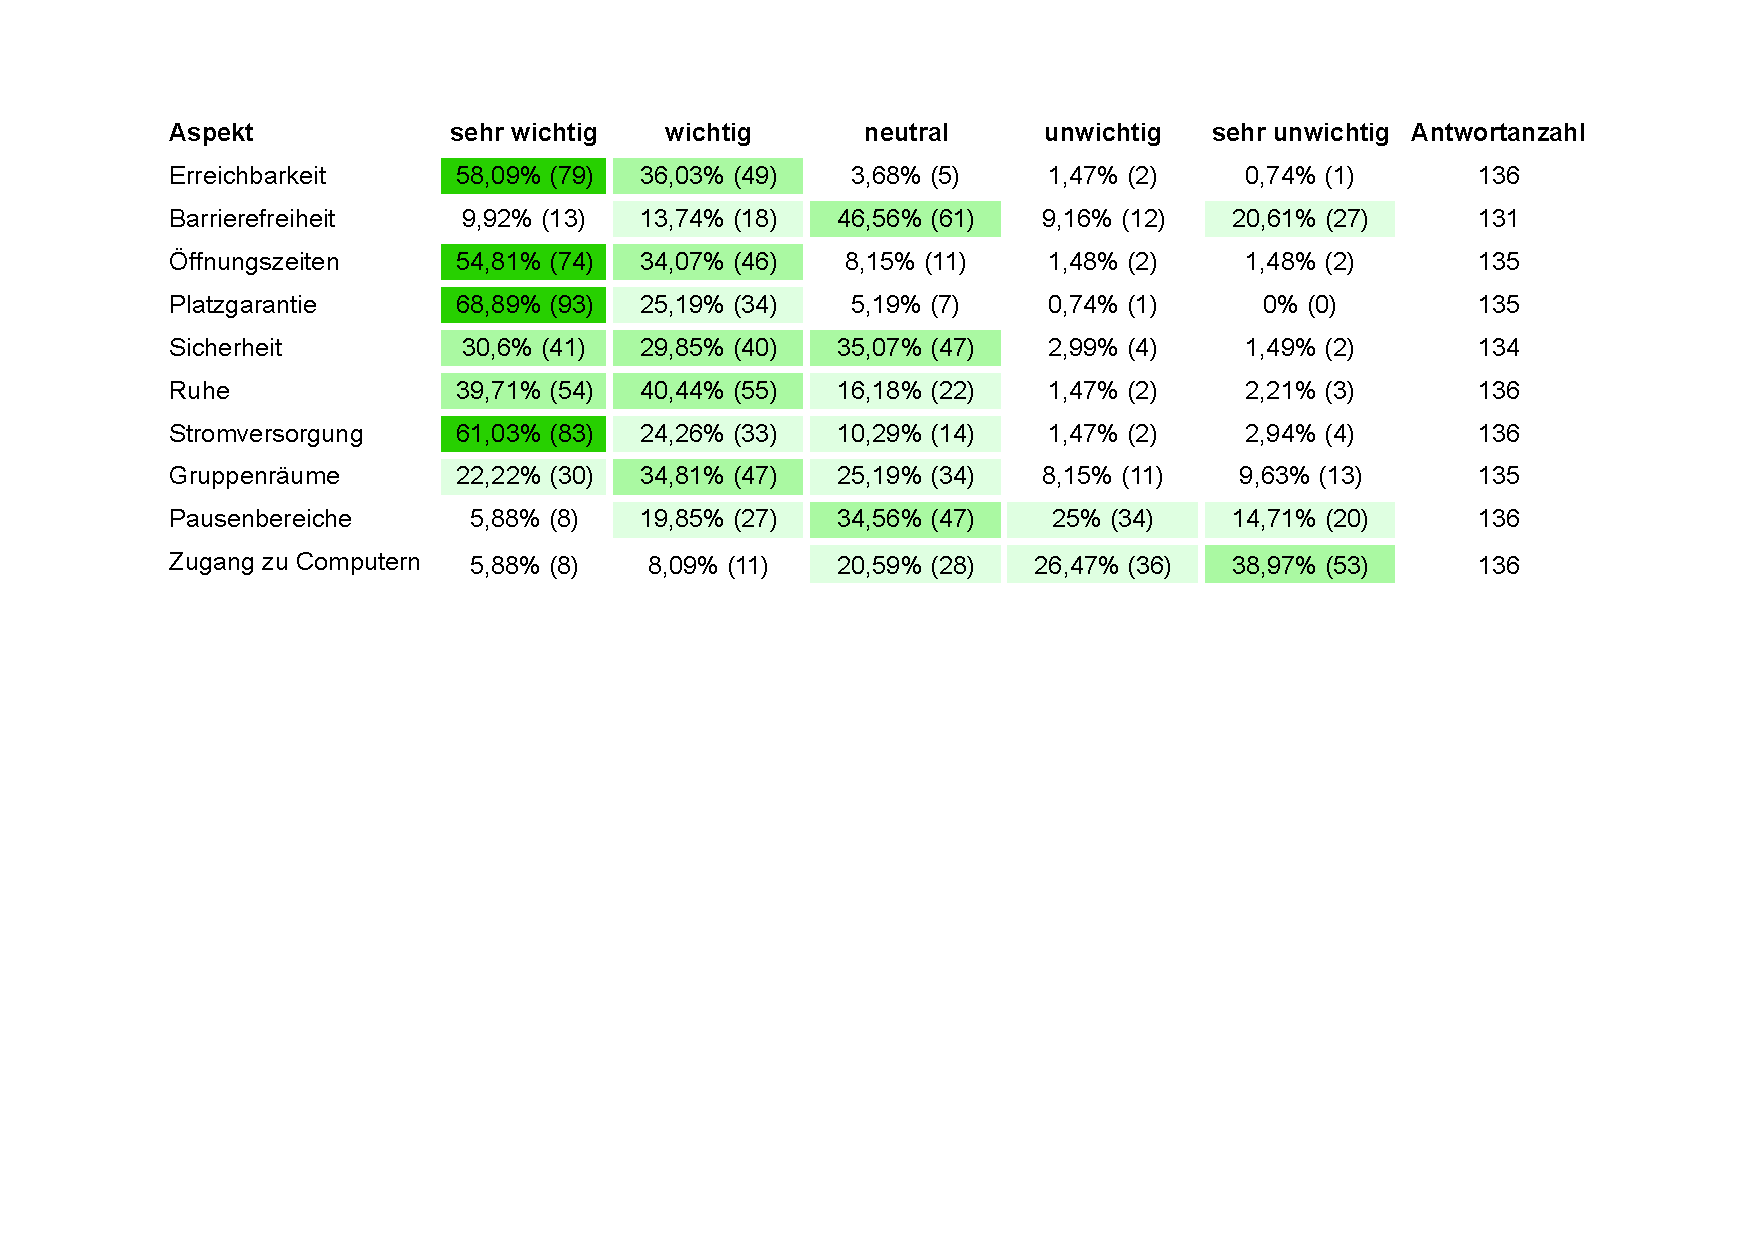
\includegraphics[scale = 0.746, trim=0.5cm 11cm 0.5cm 11cm]{Tabellen.pdf}
	\caption{Wichtigkeit der Lernorte}
	\vspace{0.5cm}
    Über 50\% der Befragten empfinden die Aspekte "'Erreichbarkeit"', "'Öffnungszeiten"', "'Platzgarantie"' und "'Stromversorgung"' als sehr wichtig. Im Gegensatz dazu ist der "'Zugang zu Computern"'  von 38.97 \% der Befragten als sehr unwichtig eingestuft.\\
	"'Ruhe"' und "'Gruppenräume"' werden größtenteils als wichtig erachtet. %von jeweils 40.44\% und 34.81\% der Befragten.\\
	Alle weiteren Aspekte, also "'Sicherheit"', "'Barrierefreiheit"' und "'Pausenbereiche"', werden eher neutral eingeschätzt.\\\\
	Die Kennzahlen der Bewertung der eben beschriebenen Aspekte werden in Tabelle 2 zusammengefasst.
\end{figure}
\centering{
\begin{table}[h]
	\vspace*{0cm}
	\hspace*{0.48cm}
	\begin{tabular}{l|cccccc}
		x                & $\bar{x}$-Vorher & $\bar{x}$-Jetzt & Differenz-$\bar{x}$ & $\tilde{x}_{0.5}$-Vorher & $\tilde{x}_{0.5}$-Jetzt & Differenz-$\tilde{x}_{0.5}$\\ \hline
		Erreichbarkeit   & 1.64              & 2.52             & 0.88                 & 2             & 2            & 0                     \\
		Barrierefreiheit & 2.22              & 2.62             & 0.40                 & 2             & 2            & 0                     \\
		Öffnungszeiten   & 1.93              & 2.79             & 0.86                 & 2             & 3            & 0                     \\
		Platzgarantie    & 2.79              & 3.61             & 0.82                 & 3             & 4            & 1                     \\
		Sicherheit       & 1.86              & 2.05             & 0.19                 & 2             & 2            & 0                     \\
		Ruhe             & 2.13              & 2.75             & 0.62                 & 2             & 3            & 1                     \\
		Stromversorgung  & 2.36              & 2.78             & 0.42                 & 2             & 3            & 1                     \\
		Gruppenräume     & 2.59              & 2.88             & 0.29                 & 3             & 3            & \multicolumn{1}{c}{0} \\
		Pausenbereiche   & 2.73              & 2.79             & 0.06                 & 3             & 3            & 0                     \\
		Computer         & 2.50              & 3.08             & 0.58                 & 2             & 3            & 1                    
	\end{tabular}
			\caption{Kennzahlen der Bewertung der Aspekte}
\end{table}
}
	\raggedright
\newpage
Die obenstehende Tabelle beinhaltet die durchschnittliche Bewertung vor dem Wintersemester 2022/ 23 sowie die Bewertung der jetzigen Situation. Im Durchschnitt werden "'Erreichbarkeit"' und "'Öffnungszeiten"' zuvor als sehr gut, die restlichen Aspekte mit gut bewertet. Im Vergleich dazu sind nach dem Wintersemester 2022/ 23 alle Aspekte, außer "'Platzgarantie"' und "'Zugang zu Computern"', die als "'befriedigend"' eingestuft werden, durchschnittlich gut bewertet worden.\\
Ebenfalls wird die Veränderung der Differenz der durchschnittlichen Bewertung angegeben. Da diese ist für alle Aspekte positiv ist, wird deutlich, dass die Bewertung für alle Aspekte schlechter geworden ist.\\
Zusätzlich wird die Veränderung des Medians der Bewertung sowie die Differenz angegeben.
Die Mediane der Aspekte sind vorher größtenteils Zwei, jetzt hingegen sind diese größtenteils Drei mit vereinzelt Zweien bzw. auch einer Vier. % komischer Satz 



\subsection{Gesamtzufriedenheit und Score}



Von großem Interesse ist in der Analyse die Gesamtzufriedenheit der Studenten mit den Lernorten.\\ Diese latente Variable haben wir, wie bereits in 3. erwähnt mit dem "'Score"' repräsentiert.
Diesen haben wir getrennt für jede einzelne Person einmal für die Situation vorher und einmal für die aktuelle Situation berechnet.
Ein niedriger Score (nahe 1) steht dabei für eine hohe Zufriedenheit und ein höherer Score stellt eine schlechtere Gesamtzufriedenheit dar.
Weiterhin is zu beachten, dass hier mit quasi-intervallskalierten Daten gerechnet wurde. \\
In Abbildung 5 wird der Score-Vorher (SV) mit dem Score-Jetzt (SJ) durch zwei Streudiagramme verglichen.
\vspace{-0.5cm}
\begin{figure}[h]
{\centering % Created by tikzDevice version 0.12.5 on 2024-01-20 15:22:02
% !TEX encoding = UTF-8 Unicode
\begin{tikzpicture}[x=1pt,y=1pt]
\definecolor{fillColor}{RGB}{255,255,255}
\path[use as bounding box,fill=fillColor,fill opacity=0.00] (0,0) rectangle (505.89,252.94);
\begin{scope}
\path[clip] ( 49.20, 61.20) rectangle (227.75,203.75);
\definecolor{fillColor}{RGB}{255,165,0}

\path[fill=fillColor] ( 55.81,178.10) circle (  2.25);

\path[fill=fillColor] ( 57.04,154.23) circle (  2.25);

\path[fill=fillColor] ( 58.26,173.50) circle (  2.25);

\path[fill=fillColor] ( 59.49,181.10) circle (  2.25);

\path[fill=fillColor] ( 60.71,198.47) circle (  2.25);
\definecolor{fillColor}{RGB}{0,0,255}

\path[fill=fillColor] ( 61.94,173.89) circle (  2.25);

\path[fill=fillColor] ( 63.16,174.40) circle (  2.25);

\path[fill=fillColor] ( 64.38,168.30) circle (  2.25);
\definecolor{fillColor}{RGB}{255,165,0}

\path[fill=fillColor] ( 65.61,165.86) circle (  2.25);

\path[fill=fillColor] ( 66.83,158.51) circle (  2.25);

\path[fill=fillColor] ( 68.06,183.80) circle (  2.25);

\path[fill=fillColor] ( 69.28,186.96) circle (  2.25);

\path[fill=fillColor] ( 70.51,188.66) circle (  2.25);

\path[fill=fillColor] ( 71.73,194.69) circle (  2.25);
\definecolor{fillColor}{RGB}{0,0,255}

\path[fill=fillColor] ( 72.96,193.67) circle (  2.25);
\definecolor{fillColor}{RGB}{255,165,0}

\path[fill=fillColor] ( 74.18,153.84) circle (  2.25);
\definecolor{fillColor}{RGB}{0,0,255}

\path[fill=fillColor] ( 75.41,154.01) circle (  2.25);
\definecolor{fillColor}{RGB}{255,165,0}

\path[fill=fillColor] ( 76.63,182.63) circle (  2.25);
\definecolor{fillColor}{RGB}{0,0,255}

\path[fill=fillColor] ( 77.86,153.31) circle (  2.25);
\definecolor{fillColor}{RGB}{255,165,0}

\path[fill=fillColor] ( 79.08,174.58) circle (  2.25);
\definecolor{fillColor}{RGB}{0,0,255}

\path[fill=fillColor] ( 80.30,188.79) circle (  2.25);

\path[fill=fillColor] ( 81.53,196.07) circle (  2.25);
\definecolor{fillColor}{RGB}{255,165,0}

\path[fill=fillColor] ( 83.98,190.29) circle (  2.25);

\path[fill=fillColor] ( 85.20,185.87) circle (  2.25);

\path[fill=fillColor] ( 86.43,158.24) circle (  2.25);

\path[fill=fillColor] ( 87.65,179.99) circle (  2.25);
\definecolor{fillColor}{RGB}{0,0,255}

\path[fill=fillColor] ( 88.88,155.66) circle (  2.25);
\definecolor{fillColor}{RGB}{255,165,0}

\path[fill=fillColor] ( 90.10,166.20) circle (  2.25);

\path[fill=fillColor] ( 91.33,165.30) circle (  2.25);

\path[fill=fillColor] ( 92.55,177.02) circle (  2.25);

\path[fill=fillColor] ( 93.78,179.44) circle (  2.25);

\path[fill=fillColor] ( 95.00,163.27) circle (  2.25);

\path[fill=fillColor] ( 96.22,160.56) circle (  2.25);

\path[fill=fillColor] ( 97.45,169.24) circle (  2.25);

\path[fill=fillColor] ( 98.67,153.84) circle (  2.25);
\definecolor{fillColor}{RGB}{0,0,255}

\path[fill=fillColor] ( 99.90,154.01) circle (  2.25);
\definecolor{fillColor}{RGB}{255,165,0}

\path[fill=fillColor] (101.12,182.63) circle (  2.25);
\definecolor{fillColor}{RGB}{0,0,255}

\path[fill=fillColor] (102.35,153.31) circle (  2.25);
\definecolor{fillColor}{RGB}{255,165,0}

\path[fill=fillColor] (103.57,174.58) circle (  2.25);

\path[fill=fillColor] (104.80,181.17) circle (  2.25);

\path[fill=fillColor] (106.02,179.01) circle (  2.25);

\path[fill=fillColor] (107.25,169.81) circle (  2.25);

\path[fill=fillColor] (108.47,154.23) circle (  2.25);

\path[fill=fillColor] (109.69,163.90) circle (  2.25);

\path[fill=fillColor] (110.92,157.67) circle (  2.25);

\path[fill=fillColor] (112.14,126.61) circle (  2.25);
\definecolor{fillColor}{RGB}{0,0,255}

\path[fill=fillColor] (113.37,148.31) circle (  2.25);
\definecolor{fillColor}{RGB}{255,165,0}

\path[fill=fillColor] (114.59,196.76) circle (  2.25);

\path[fill=fillColor] (115.82,162.79) circle (  2.25);
\definecolor{fillColor}{RGB}{0,0,255}

\path[fill=fillColor] (117.04,188.25) circle (  2.25);
\definecolor{fillColor}{RGB}{255,165,0}

\path[fill=fillColor] (118.27,172.07) circle (  2.25);

\path[fill=fillColor] (119.49,140.11) circle (  2.25);

\path[fill=fillColor] (120.72,162.17) circle (  2.25);

\path[fill=fillColor] (121.94,180.55) circle (  2.25);

\path[fill=fillColor] (123.17,158.87) circle (  2.25);

\path[fill=fillColor] (124.39,116.87) circle (  2.25);

\path[fill=fillColor] (125.61,166.41) circle (  2.25);

\path[fill=fillColor] (126.84,169.05) circle (  2.25);

\path[fill=fillColor] (128.06,164.00) circle (  2.25);

\path[fill=fillColor] (129.29,171.24) circle (  2.25);

\path[fill=fillColor] (130.51,198.47) circle (  2.25);
\definecolor{fillColor}{RGB}{0,0,255}

\path[fill=fillColor] (131.74,167.04) circle (  2.25);
\definecolor{fillColor}{RGB}{255,165,0}

\path[fill=fillColor] (132.96,176.93) circle (  2.25);
\definecolor{fillColor}{RGB}{0,0,255}

\path[fill=fillColor] (134.19,177.35) circle (  2.25);
\definecolor{fillColor}{RGB}{255,165,0}

\path[fill=fillColor] (135.41,185.90) circle (  2.25);
\definecolor{fillColor}{RGB}{0,0,255}

\path[fill=fillColor] (136.64,152.44) circle (  2.25);
\definecolor{fillColor}{RGB}{255,165,0}

\path[fill=fillColor] (137.86,180.87) circle (  2.25);

\path[fill=fillColor] (140.31,140.39) circle (  2.25);

\path[fill=fillColor] (141.53,183.38) circle (  2.25);
\definecolor{fillColor}{RGB}{0,0,255}

\path[fill=fillColor] (142.76,174.54) circle (  2.25);
\definecolor{fillColor}{RGB}{255,165,0}

\path[fill=fillColor] (143.98,169.87) circle (  2.25);

\path[fill=fillColor] (145.21,167.67) circle (  2.25);
\definecolor{fillColor}{RGB}{0,0,255}

\path[fill=fillColor] (146.43,194.60) circle (  2.25);
\definecolor{fillColor}{RGB}{255,165,0}

\path[fill=fillColor] (147.66,158.18) circle (  2.25);

\path[fill=fillColor] (148.88,159.15) circle (  2.25);

\path[fill=fillColor] (150.11,157.40) circle (  2.25);

\path[fill=fillColor] (151.33,146.45) circle (  2.25);

\path[fill=fillColor] (152.56,161.37) circle (  2.25);

\path[fill=fillColor] (153.78,191.13) circle (  2.25);

\path[fill=fillColor] (155.00,183.48) circle (  2.25);

\path[fill=fillColor] (156.23,152.93) circle (  2.25);
\definecolor{fillColor}{RGB}{0,0,255}

\path[fill=fillColor] (157.45,157.22) circle (  2.25);
\definecolor{fillColor}{RGB}{255,165,0}

\path[fill=fillColor] (158.68,161.85) circle (  2.25);

\path[fill=fillColor] (159.90,161.07) circle (  2.25);

\path[fill=fillColor] (161.13,154.77) circle (  2.25);

\path[fill=fillColor] (162.35,156.74) circle (  2.25);

\path[fill=fillColor] (163.58,163.04) circle (  2.25);
\definecolor{fillColor}{RGB}{0,0,255}

\path[fill=fillColor] (164.80,161.65) circle (  2.25);
\definecolor{fillColor}{RGB}{255,165,0}

\path[fill=fillColor] (166.03,142.96) circle (  2.25);

\path[fill=fillColor] (167.25,131.34) circle (  2.25);

\path[fill=fillColor] (168.47,164.30) circle (  2.25);

\path[fill=fillColor] (169.70,150.07) circle (  2.25);

\path[fill=fillColor] (170.92,167.56) circle (  2.25);

\path[fill=fillColor] (172.15,155.66) circle (  2.25);

\path[fill=fillColor] (173.37,174.78) circle (  2.25);
\definecolor{fillColor}{RGB}{0,0,255}

\path[fill=fillColor] (174.60,180.61) circle (  2.25);

\path[fill=fillColor] (175.82,162.79) circle (  2.25);
\definecolor{fillColor}{RGB}{255,165,0}

\path[fill=fillColor] (177.05,165.47) circle (  2.25);
\definecolor{fillColor}{RGB}{0,0,255}

\path[fill=fillColor] (178.27,173.42) circle (  2.25);
\definecolor{fillColor}{RGB}{255,165,0}

\path[fill=fillColor] (179.50,167.79) circle (  2.25);

\path[fill=fillColor] (180.72,175.84) circle (  2.25);

\path[fill=fillColor] (181.95,160.65) circle (  2.25);

\path[fill=fillColor] (183.17,160.26) circle (  2.25);
\definecolor{fillColor}{RGB}{0,0,255}

\path[fill=fillColor] (184.39,172.71) circle (  2.25);
\definecolor{fillColor}{RGB}{255,165,0}

\path[fill=fillColor] (185.62,172.71) circle (  2.25);

\path[fill=fillColor] (186.84,175.37) circle (  2.25);

\path[fill=fillColor] (188.07,115.11) circle (  2.25);

\path[fill=fillColor] (189.29,127.34) circle (  2.25);

\path[fill=fillColor] (190.52,178.51) circle (  2.25);

\path[fill=fillColor] (191.74,170.56) circle (  2.25);

\path[fill=fillColor] (192.97,188.37) circle (  2.25);

\path[fill=fillColor] (194.19,145.06) circle (  2.25);

\path[fill=fillColor] (195.42,169.49) circle (  2.25);
\definecolor{fillColor}{RGB}{0,0,255}

\path[fill=fillColor] (196.64,166.27) circle (  2.25);
\definecolor{fillColor}{RGB}{255,165,0}

\path[fill=fillColor] (197.87,141.71) circle (  2.25);

\path[fill=fillColor] (199.09,188.02) circle (  2.25);

\path[fill=fillColor] (200.31,173.91) circle (  2.25);
\definecolor{fillColor}{RGB}{0,0,255}

\path[fill=fillColor] (201.54,128.55) circle (  2.25);
\definecolor{fillColor}{RGB}{255,165,0}

\path[fill=fillColor] (202.76,176.35) circle (  2.25);

\path[fill=fillColor] (203.99,172.75) circle (  2.25);

\path[fill=fillColor] (205.21,174.05) circle (  2.25);

\path[fill=fillColor] (206.44,155.87) circle (  2.25);

\path[fill=fillColor] (207.66,179.92) circle (  2.25);
\definecolor{fillColor}{RGB}{0,0,255}

\path[fill=fillColor] (208.89,166.41) circle (  2.25);

\path[fill=fillColor] (210.11,157.67) circle (  2.25);
\definecolor{fillColor}{RGB}{255,165,0}

\path[fill=fillColor] (211.34,155.82) circle (  2.25);

\path[fill=fillColor] (212.56,151.47) circle (  2.25);

\path[fill=fillColor] (213.78,140.39) circle (  2.25);

\path[fill=fillColor] (215.01,148.45) circle (  2.25);
\definecolor{fillColor}{RGB}{0,0,255}

\path[fill=fillColor] (216.23,185.27) circle (  2.25);
\definecolor{fillColor}{RGB}{255,165,0}

\path[fill=fillColor] (217.46,173.39) circle (  2.25);

\path[fill=fillColor] (218.68,163.02) circle (  2.25);

\path[fill=fillColor] (219.91,152.87) circle (  2.25);
\definecolor{fillColor}{RGB}{0,0,255}

\path[fill=fillColor] (221.13,154.19) circle (  2.25);
\end{scope}
\begin{scope}
\path[clip] (  0.00,  0.00) rectangle (505.89,252.94);
\definecolor{drawColor}{RGB}{0,0,0}

\path[draw=drawColor,line width= 0.4pt,line join=round,line cap=round] ( 49.20,198.47) -- ( 49.20, 66.48);

\path[draw=drawColor,line width= 0.4pt,line join=round,line cap=round] ( 49.20,198.47) -- ( 43.20,198.47);

\path[draw=drawColor,line width= 0.4pt,line join=round,line cap=round] ( 49.20,172.07) -- ( 43.20,172.07);

\path[draw=drawColor,line width= 0.4pt,line join=round,line cap=round] ( 49.20,145.67) -- ( 43.20,145.67);

\path[draw=drawColor,line width= 0.4pt,line join=round,line cap=round] ( 49.20,119.27) -- ( 43.20,119.27);

\path[draw=drawColor,line width= 0.4pt,line join=round,line cap=round] ( 49.20, 92.88) -- ( 43.20, 92.88);

\path[draw=drawColor,line width= 0.4pt,line join=round,line cap=round] ( 49.20, 66.48) -- ( 43.20, 66.48);

\node[text=drawColor,rotate= 90.00,anchor=base,inner sep=0pt, outer sep=0pt, scale=  1.00] at ( 34.80, 66.48) {6};

\node[text=drawColor,rotate= 90.00,anchor=base,inner sep=0pt, outer sep=0pt, scale=  1.00] at ( 34.80, 92.88) {5};

\node[text=drawColor,rotate= 90.00,anchor=base,inner sep=0pt, outer sep=0pt, scale=  1.00] at ( 34.80,119.27) {4};

\node[text=drawColor,rotate= 90.00,anchor=base,inner sep=0pt, outer sep=0pt, scale=  1.00] at ( 34.80,145.67) {3};

\node[text=drawColor,rotate= 90.00,anchor=base,inner sep=0pt, outer sep=0pt, scale=  1.00] at ( 34.80,172.07) {2};

\node[text=drawColor,rotate= 90.00,anchor=base,inner sep=0pt, outer sep=0pt, scale=  1.00] at ( 34.80,198.47) {1};

\path[draw=drawColor,line width= 0.4pt,line join=round,line cap=round] ( 49.20, 61.20) --
	(227.75, 61.20) --
	(227.75,203.75) --
	( 49.20,203.75) --
	cycle;
\end{scope}
\begin{scope}
\path[clip] (  0.00,  0.00) rectangle (252.94,252.94);
\definecolor{drawColor}{RGB}{0,0,0}

\node[text=drawColor,anchor=base,inner sep=0pt, outer sep=0pt, scale=  1.20] at (138.47,224.20) {\bfseries Score Vorher};

\node[text=drawColor,rotate= 90.00,anchor=base,inner sep=0pt, outer sep=0pt, scale=  1.00] at ( 10.80,132.47) {Score Vorher};
\end{scope}
\begin{scope}
\path[clip] ( 49.20, 61.20) rectangle (227.75,203.75);
\definecolor{drawColor}{RGB}{255,0,0}

\path[draw=drawColor,line width= 1.2pt,line join=round,line cap=round] ( 49.20,166.62) -- (227.74,166.62);
\end{scope}
\begin{scope}
\path[clip] (302.14, 61.20) rectangle (480.69,203.75);
\definecolor{fillColor}{RGB}{255,165,0}

\path[fill=fillColor] (308.76,156.98) circle (  2.25);

\path[fill=fillColor] (309.98,150.67) circle (  2.25);

\path[fill=fillColor] (311.21,137.82) circle (  2.25);

\path[fill=fillColor] (312.43,144.98) circle (  2.25);

\path[fill=fillColor] (313.66,119.90) circle (  2.25);
\definecolor{fillColor}{RGB}{0,0,255}

\path[fill=fillColor] (314.88,173.89) circle (  2.25);

\path[fill=fillColor] (316.11,174.40) circle (  2.25);

\path[fill=fillColor] (317.33,153.84) circle (  2.25);
\definecolor{fillColor}{RGB}{255,165,0}

\path[fill=fillColor] (318.55,144.89) circle (  2.25);

\path[fill=fillColor] (319.78,154.23) circle (  2.25);

\path[fill=fillColor] (321.00,154.47) circle (  2.25);

\path[fill=fillColor] (322.23,149.06) circle (  2.25);

\path[fill=fillColor] (323.45,160.00) circle (  2.25);

\path[fill=fillColor] (324.68,165.78) circle (  2.25);
\definecolor{fillColor}{RGB}{0,0,255}

\path[fill=fillColor] (325.90,193.67) circle (  2.25);
\definecolor{fillColor}{RGB}{255,165,0}

\path[fill=fillColor] (327.13,153.84) circle (  2.25);
\definecolor{fillColor}{RGB}{0,0,255}

\path[fill=fillColor] (328.35,150.53) circle (  2.25);
\definecolor{fillColor}{RGB}{255,165,0}

\path[fill=fillColor] (329.58,129.83) circle (  2.25);
\definecolor{fillColor}{RGB}{0,0,255}

\path[fill=fillColor] (330.80,139.42) circle (  2.25);
\definecolor{fillColor}{RGB}{255,165,0}

\path[fill=fillColor] (332.02,175.84) circle (  2.25);
\definecolor{fillColor}{RGB}{0,0,255}

\path[fill=fillColor] (333.25,188.79) circle (  2.25);

\path[fill=fillColor] (334.47,196.07) circle (  2.25);
\definecolor{fillColor}{RGB}{255,165,0}

\path[fill=fillColor] (336.92,177.10) circle (  2.25);

\path[fill=fillColor] (338.15,172.67) circle (  2.25);

\path[fill=fillColor] (339.37,148.81) circle (  2.25);

\path[fill=fillColor] (340.60,146.99) circle (  2.25);
\definecolor{fillColor}{RGB}{0,0,255}

\path[fill=fillColor] (341.82,152.81) circle (  2.25);
\definecolor{fillColor}{RGB}{255,165,0}

\path[fill=fillColor] (343.05,160.92) circle (  2.25);

\path[fill=fillColor] (344.27,138.23) circle (  2.25);

\path[fill=fillColor] (345.50,147.32) circle (  2.25);

\path[fill=fillColor] (346.72,145.06) circle (  2.25);

\path[fill=fillColor] (347.94,128.75) circle (  2.25);

\path[fill=fillColor] (349.17,176.13) circle (  2.25);

\path[fill=fillColor] (350.39,169.24) circle (  2.25);

\path[fill=fillColor] (351.62,153.84) circle (  2.25);
\definecolor{fillColor}{RGB}{0,0,255}

\path[fill=fillColor] (352.84,150.53) circle (  2.25);
\definecolor{fillColor}{RGB}{255,165,0}

\path[fill=fillColor] (354.07,129.83) circle (  2.25);
\definecolor{fillColor}{RGB}{0,0,255}

\path[fill=fillColor] (355.29,139.42) circle (  2.25);
\definecolor{fillColor}{RGB}{255,165,0}

\path[fill=fillColor] (356.52,175.84) circle (  2.25);

\path[fill=fillColor] (357.74,168.43) circle (  2.25);

\path[fill=fillColor] (358.97,176.93) circle (  2.25);

\path[fill=fillColor] (360.19,148.69) circle (  2.25);

\path[fill=fillColor] (361.42,147.10) circle (  2.25);

\path[fill=fillColor] (362.64,147.56) circle (  2.25);

\path[fill=fillColor] (363.86,168.07) circle (  2.25);

\path[fill=fillColor] (365.09,106.08) circle (  2.25);
\definecolor{fillColor}{RGB}{0,0,255}

\path[fill=fillColor] (366.31,148.31) circle (  2.25);
\definecolor{fillColor}{RGB}{255,165,0}

\path[fill=fillColor] (367.54,126.94) circle (  2.25);

\path[fill=fillColor] (368.76,142.82) circle (  2.25);
\definecolor{fillColor}{RGB}{0,0,255}

\path[fill=fillColor] (369.99,188.25) circle (  2.25);
\definecolor{fillColor}{RGB}{255,165,0}

\path[fill=fillColor] (371.21, 92.88) circle (  2.25);

\path[fill=fillColor] (372.44,119.27) circle (  2.25);

\path[fill=fillColor] (373.66,158.87) circle (  2.25);

\path[fill=fillColor] (374.89,124.93) circle (  2.25);

\path[fill=fillColor] (376.11,150.29) circle (  2.25);

\path[fill=fillColor] (377.33,118.67) circle (  2.25);

\path[fill=fillColor] (378.56,146.93) circle (  2.25);

\path[fill=fillColor] (379.78,141.90) circle (  2.25);

\path[fill=fillColor] (381.01,132.47) circle (  2.25);

\path[fill=fillColor] (382.23,167.12) circle (  2.25);

\path[fill=fillColor] (383.46,158.87) circle (  2.25);
\definecolor{fillColor}{RGB}{0,0,255}

\path[fill=fillColor] (384.68,176.47) circle (  2.25);
\definecolor{fillColor}{RGB}{255,165,0}

\path[fill=fillColor] (385.91,183.88) circle (  2.25);
\definecolor{fillColor}{RGB}{0,0,255}

\path[fill=fillColor] (387.13,177.35) circle (  2.25);
\definecolor{fillColor}{RGB}{255,165,0}

\path[fill=fillColor] (388.36,122.42) circle (  2.25);
\definecolor{fillColor}{RGB}{0,0,255}

\path[fill=fillColor] (389.58,155.82) circle (  2.25);
\definecolor{fillColor}{RGB}{255,165,0}

\path[fill=fillColor] (390.81,164.00) circle (  2.25);
\definecolor{fillColor}{RGB}{0,0,255}

\path[fill=fillColor] (392.03,172.07) circle (  2.25);
\definecolor{fillColor}{RGB}{255,165,0}

\path[fill=fillColor] (393.25,140.39) circle (  2.25);

\path[fill=fillColor] (394.48,159.50) circle (  2.25);
\definecolor{fillColor}{RGB}{0,0,255}

\path[fill=fillColor] (395.70,174.54) circle (  2.25);
\definecolor{fillColor}{RGB}{255,165,0}

\path[fill=fillColor] (396.93,151.54) circle (  2.25);

\path[fill=fillColor] (398.15,165.91) circle (  2.25);
\definecolor{fillColor}{RGB}{0,0,255}

\path[fill=fillColor] (399.38,198.47) circle (  2.25);
\definecolor{fillColor}{RGB}{255,165,0}

\path[fill=fillColor] (400.60,158.18) circle (  2.25);

\path[fill=fillColor] (401.83,156.90) circle (  2.25);

\path[fill=fillColor] (403.05,148.60) circle (  2.25);

\path[fill=fillColor] (404.28,141.79) circle (  2.25);

\path[fill=fillColor] (405.50,161.37) circle (  2.25);

\path[fill=fillColor] (406.72,174.27) circle (  2.25);

\path[fill=fillColor] (407.95,167.79) circle (  2.25);

\path[fill=fillColor] (409.17,143.03) circle (  2.25);
\definecolor{fillColor}{RGB}{0,0,255}

\path[fill=fillColor] (410.40,150.62) circle (  2.25);
\definecolor{fillColor}{RGB}{255,165,0}

\path[fill=fillColor] (411.62,148.23) circle (  2.25);

\path[fill=fillColor] (412.85,145.67) circle (  2.25);

\path[fill=fillColor] (414.07,142.94) circle (  2.25);

\path[fill=fillColor] (415.30,149.93) circle (  2.25);

\path[fill=fillColor] (416.52,160.95) circle (  2.25);
\definecolor{fillColor}{RGB}{0,0,255}

\path[fill=fillColor] (417.75,161.65) circle (  2.25);
\definecolor{fillColor}{RGB}{255,165,0}

\path[fill=fillColor] (418.97,149.73) circle (  2.25);

\path[fill=fillColor] (420.20,101.93) circle (  2.25);

\path[fill=fillColor] (421.42,137.13) circle (  2.25);

\path[fill=fillColor] (422.64,148.31) circle (  2.25);

\path[fill=fillColor] (423.87,153.40) circle (  2.25);

\path[fill=fillColor] (425.09,149.95) circle (  2.25);

\path[fill=fillColor] (426.32,147.02) circle (  2.25);
\definecolor{fillColor}{RGB}{0,0,255}

\path[fill=fillColor] (427.54,171.29) circle (  2.25);

\path[fill=fillColor] (428.77,167.07) circle (  2.25);
\definecolor{fillColor}{RGB}{255,165,0}

\path[fill=fillColor] (429.99,144.20) circle (  2.25);
\definecolor{fillColor}{RGB}{0,0,255}

\path[fill=fillColor] (431.22,170.04) circle (  2.25);
\definecolor{fillColor}{RGB}{255,165,0}

\path[fill=fillColor] (432.44,155.66) circle (  2.25);

\path[fill=fillColor] (433.67,162.26) circle (  2.25);

\path[fill=fillColor] (434.89,149.24) circle (  2.25);

\path[fill=fillColor] (436.11,158.18) circle (  2.25);
\definecolor{fillColor}{RGB}{0,0,255}

\path[fill=fillColor] (437.34,148.89) circle (  2.25);
\definecolor{fillColor}{RGB}{255,165,0}

\path[fill=fillColor] (438.56,148.89) circle (  2.25);

\path[fill=fillColor] (439.79,139.90) circle (  2.25);

\path[fill=fillColor] (441.01,103.30) circle (  2.25);

\path[fill=fillColor] (442.24, 94.34) circle (  2.25);

\path[fill=fillColor] (443.46,154.04) circle (  2.25);

\path[fill=fillColor] (444.69,123.04) circle (  2.25);

\path[fill=fillColor] (445.91,117.72) circle (  2.25);

\path[fill=fillColor] (447.14,125.41) circle (  2.25);

\path[fill=fillColor] (448.36,153.40) circle (  2.25);
\definecolor{fillColor}{RGB}{0,0,255}

\path[fill=fillColor] (449.59,168.85) circle (  2.25);
\definecolor{fillColor}{RGB}{255,165,0}

\path[fill=fillColor] (450.81,141.71) circle (  2.25);

\path[fill=fillColor] (452.03,190.77) circle (  2.25);

\path[fill=fillColor] (453.26,146.90) circle (  2.25);
\definecolor{fillColor}{RGB}{0,0,255}

\path[fill=fillColor] (454.48,122.84) circle (  2.25);
\definecolor{fillColor}{RGB}{255,165,0}

\path[fill=fillColor] (455.71,194.18) circle (  2.25);

\path[fill=fillColor] (456.93,159.21) circle (  2.25);

\path[fill=fillColor] (458.16,173.39) circle (  2.25);

\path[fill=fillColor] (459.38,143.87) circle (  2.25);

\path[fill=fillColor] (460.61,155.66) circle (  2.25);
\definecolor{fillColor}{RGB}{0,0,255}

\path[fill=fillColor] (461.83,166.41) circle (  2.25);

\path[fill=fillColor] (463.06,157.67) circle (  2.25);
\definecolor{fillColor}{RGB}{255,165,0}

\path[fill=fillColor] (464.28,132.81) circle (  2.25);

\path[fill=fillColor] (465.51,163.05) circle (  2.25);

\path[fill=fillColor] (466.73,130.49) circle (  2.25);

\path[fill=fillColor] (467.95,158.18) circle (  2.25);
\definecolor{fillColor}{RGB}{0,0,255}

\path[fill=fillColor] (469.18,176.73) circle (  2.25);
\definecolor{fillColor}{RGB}{255,165,0}

\path[fill=fillColor] (470.40,150.29) circle (  2.25);

\path[fill=fillColor] (471.63,139.64) circle (  2.25);

\path[fill=fillColor] (472.85,168.07) circle (  2.25);
\definecolor{fillColor}{RGB}{0,0,255}

\path[fill=fillColor] (474.08,150.78) circle (  2.25);
\end{scope}
\begin{scope}
\path[clip] (  0.00,  0.00) rectangle (505.89,252.94);
\definecolor{drawColor}{RGB}{0,0,0}

\path[draw=drawColor,line width= 0.4pt,line join=round,line cap=round] (302.14,198.47) -- (302.14, 66.48);

\path[draw=drawColor,line width= 0.4pt,line join=round,line cap=round] (302.14,198.47) -- (296.14,198.47);

\path[draw=drawColor,line width= 0.4pt,line join=round,line cap=round] (302.14,172.07) -- (296.14,172.07);

\path[draw=drawColor,line width= 0.4pt,line join=round,line cap=round] (302.14,145.67) -- (296.14,145.67);

\path[draw=drawColor,line width= 0.4pt,line join=round,line cap=round] (302.14,119.27) -- (296.14,119.27);

\path[draw=drawColor,line width= 0.4pt,line join=round,line cap=round] (302.14, 92.88) -- (296.14, 92.88);

\path[draw=drawColor,line width= 0.4pt,line join=round,line cap=round] (302.14, 66.48) -- (296.14, 66.48);

\node[text=drawColor,rotate= 90.00,anchor=base,inner sep=0pt, outer sep=0pt, scale=  1.00] at (287.75, 66.48) {6};

\node[text=drawColor,rotate= 90.00,anchor=base,inner sep=0pt, outer sep=0pt, scale=  1.00] at (287.75, 92.88) {5};

\node[text=drawColor,rotate= 90.00,anchor=base,inner sep=0pt, outer sep=0pt, scale=  1.00] at (287.75,119.27) {4};

\node[text=drawColor,rotate= 90.00,anchor=base,inner sep=0pt, outer sep=0pt, scale=  1.00] at (287.75,145.67) {3};

\node[text=drawColor,rotate= 90.00,anchor=base,inner sep=0pt, outer sep=0pt, scale=  1.00] at (287.75,172.07) {2};

\node[text=drawColor,rotate= 90.00,anchor=base,inner sep=0pt, outer sep=0pt, scale=  1.00] at (287.75,198.47) {1};

\path[draw=drawColor,line width= 0.4pt,line join=round,line cap=round] (302.14, 61.20) --
	(480.69, 61.20) --
	(480.69,203.75) --
	(302.14,203.75) --
	cycle;
\end{scope}
\begin{scope}
\path[clip] (252.94,  0.00) rectangle (505.89,252.94);
\definecolor{drawColor}{RGB}{0,0,0}

\node[text=drawColor,anchor=base,inner sep=0pt, outer sep=0pt, scale=  1.20] at (391.42,224.20) {\bfseries Score Nachher};

\node[text=drawColor,rotate= 90.00,anchor=base,inner sep=0pt, outer sep=0pt, scale=  1.00] at (263.75,132.47) {Score Nachher};
\end{scope}
\begin{scope}
\path[clip] (302.14, 61.20) rectangle (480.69,203.75);
\definecolor{drawColor}{RGB}{255,0,0}

\path[draw=drawColor,line width= 1.2pt,line join=round,line cap=round] (302.14,152.47) -- (480.69,152.47);
\end{scope}
\end{tikzpicture}

\vspace{-1.8cm}
\caption{Streudiagramme zu Score Vorher und Jetzt}}
\vspace{1cm}
Dabei wird mit Orange gekennzeichnet, welche Studierende tatsächlich die UB benutzt haben. Die rote Gerade entspricht dem Mittelwert der jeweiligen Scores. \\
Direkt erkennbar ist, dass die Punkte im linken Diagramm deutlich höher und somit näher an der 1. liegen als die Punkte im SJ Diagramm.
Ebenso auffällig ist, dass auch die rote Horizontale einen niedriger Wert für Vorher darstellt. 
Von vorher zu aktuell ist hier ein klar negativer Trend zu erkennen.
Im rechten Diagramm ist bei genauerer Betrachtung zu sehen, dass sich vor allem die Orangen Punkte unter der roten Mittelwert-Geraden liegen.
Grob erscheint es auch so, als würden die Punkte im Streudiagramm SJ mehr streuen, als die im "'Score-Vorher"'.\\\\
\end{figure}
\newpage
Um diese Aussage anhand der Stichprobe zu bestätigen vergleichen wir anhand folgender Tabelle die statistischen Kennzahlen der beiden Variablen Score-Vorher und Score-Jetzt: 



\begin{table}[h]
	\vspace{0.2cm}
	\centering
	\begin{tabular}{c|ccccccccc|c}
		x & $\bar{x}$ & $s_x^2$ & $s_x$ & $min_x$ & $\tilde{x}_{0.25}$ & $\tilde{x}$ & $\tilde{x}_{0.75}$ & $max_x$ & $IQA$ & $n$ \\ \hline
		Score-Vorher & 2.20 & 0.39 & 0.62 & 1.00 & 1.78 & 2.20 & 2.61 & 4.16 & 0.83 & 136 \\
		Score-Jetzt & 2.74 & 0.57 & 0.76 & 1.00 & 2.24 & 2.81 & 3.10 & 5.00 & 0.86 & 136
	\end{tabular}
	\caption{Übersicht Score}
\end{table}
	Die Kennzahlen bestätigen den Eindruck der Streudiagramme:\\
Das arithmetische Mittel $\bar{x}$ ist beim Score Vorher kleiner.
Auch die Streuung um $\bar{x}$ ist wie bereits angenommen beim Score-Vorher kleiner. Auch die 25\%- und 75\%-Quantile erhalten bei Score-Jetzt einen höheren Wert eben so wie der Median $\tilde{x}$.
Der Interquantilabstand ist bei beiden Variablen fast identisch. \\
	Zuletzt möchten wir die Differenz: SV-SJ betrachten. Ein negativer Wert stellt also eine zeitliche Verschlechterung des Scores da.
Diese wird hier in Abhängigkeit zur durchschnittlichen Fahrzeit der Studierenden visualisiert.
\begin{figure}[h]
	{\centering % Created by tikzDevice version 0.12.6 on 2024-01-22 20:56:20
% !TEX encoding = UTF-8 Unicode
\begin{tikzpicture}[x=1pt,y=1pt]
\definecolor{fillColor}{RGB}{255,255,255}
\path[use as bounding box,fill=fillColor,fill opacity=0.00] (0,0) rectangle (505.89,252.94);
\begin{scope}
\path[clip] ( 49.20, 61.20) rectangle (480.69,203.75);
\definecolor{drawColor}{RGB}{0,0,139}

\path[draw=drawColor,line width= 0.4pt,line join=round,line cap=round] (301.27,114.87) circle (  2.25);

\path[draw=drawColor,line width= 0.4pt,line join=round,line cap=round] (174.14,129.50) circle (  2.25);

\path[draw=drawColor,line width= 0.4pt,line join=round,line cap=round] (137.82,102.75) circle (  2.25);

\path[draw=drawColor,line width= 0.4pt,line join=round,line cap=round] (137.82,102.37) circle (  2.25);

\path[draw=drawColor,line width= 0.4pt,line join=round,line cap=round] (119.66, 67.00) circle (  2.25);

\path[draw=drawColor,line width= 0.4pt,line join=round,line cap=round] (119.66,132.47) circle (  2.25);

\path[draw=drawColor,line width= 0.4pt,line join=round,line cap=round] (192.30,132.47) circle (  2.25);

\path[draw=drawColor,line width= 0.4pt,line join=round,line cap=round] (210.46,120.43) circle (  2.25);

\path[draw=drawColor,line width= 0.4pt,line join=round,line cap=round] (155.98,115.00) circle (  2.25);

\path[draw=drawColor,line width= 0.4pt,line join=round,line cap=round] (101.50,128.91) circle (  2.25);

\path[draw=drawColor,line width= 0.4pt,line join=round,line cap=round] (155.98,108.03) circle (  2.25);

\path[draw=drawColor,line width= 0.4pt,line join=round,line cap=round] (155.98,100.89) circle (  2.25);

\path[draw=drawColor,line width= 0.4pt,line join=round,line cap=round] (137.82,108.59) circle (  2.25);

\path[draw=drawColor,line width= 0.4pt,line join=round,line cap=round] (155.98,108.38) circle (  2.25);

\path[draw=drawColor,line width= 0.4pt,line join=round,line cap=round] (210.46,132.47) circle (  2.25);

\path[draw=drawColor,line width= 0.4pt,line join=round,line cap=round] (174.14,132.47) circle (  2.25);

\path[draw=drawColor,line width= 0.4pt,line join=round,line cap=round] (174.14,129.58) circle (  2.25);

\path[draw=drawColor,line width= 0.4pt,line join=round,line cap=round] (137.82, 88.48) circle (  2.25);

\path[draw=drawColor,line width= 0.4pt,line join=round,line cap=round] (155.98,120.89) circle (  2.25);

\path[draw=drawColor,line width= 0.4pt,line join=round,line cap=round] (137.82,133.52) circle (  2.25);

\path[draw=drawColor,line width= 0.4pt,line join=round,line cap=round] (228.62,132.47) circle (  2.25);

\path[draw=drawColor,line width= 0.4pt,line join=round,line cap=round] (192.30,132.47) circle (  2.25);

\path[draw=drawColor,line width= 0.4pt,line join=round,line cap=round] (192.30,121.47) circle (  2.25);

\path[draw=drawColor,line width= 0.4pt,line join=round,line cap=round] (155.98,121.47) circle (  2.25);

\path[draw=drawColor,line width= 0.4pt,line join=round,line cap=round] ( 83.34,124.62) circle (  2.25);

\path[draw=drawColor,line width= 0.4pt,line join=round,line cap=round] (210.46,104.98) circle (  2.25);

\path[draw=drawColor,line width= 0.4pt,line join=round,line cap=round] ( 76.08,130.09) circle (  2.25);

\path[draw=drawColor,line width= 0.4pt,line join=round,line cap=round] (101.50,128.07) circle (  2.25);

\path[draw=drawColor,line width= 0.4pt,line join=round,line cap=round] ( 90.61,109.91) circle (  2.25);

\path[draw=drawColor,line width= 0.4pt,line join=round,line cap=round] (192.30,107.73) circle (  2.25);

\path[draw=drawColor,line width= 0.4pt,line join=round,line cap=round] (119.66,103.82) circle (  2.25);

\path[draw=drawColor,line width= 0.4pt,line join=round,line cap=round] (174.14,103.71) circle (  2.25);

\path[draw=drawColor,line width= 0.4pt,line join=round,line cap=round] (101.50,145.45) circle (  2.25);

\path[draw=drawColor,line width= 0.4pt,line join=round,line cap=round] (174.14,132.47) circle (  2.25);

\path[draw=drawColor,line width= 0.4pt,line join=round,line cap=round] (119.66,132.47) circle (  2.25);

\path[draw=drawColor,line width= 0.4pt,line join=round,line cap=round] (283.11,129.58) circle (  2.25);

\path[draw=drawColor,line width= 0.4pt,line join=round,line cap=round] (101.50, 88.48) circle (  2.25);

\path[draw=drawColor,line width= 0.4pt,line join=round,line cap=round] (174.14,120.89) circle (  2.25);

\path[draw=drawColor,line width= 0.4pt,line join=round,line cap=round] (174.14,133.52) circle (  2.25);

\path[draw=drawColor,line width= 0.4pt,line join=round,line cap=round] (192.30,121.85) circle (  2.25);

\path[draw=drawColor,line width= 0.4pt,line join=round,line cap=round] (228.62,130.74) circle (  2.25);

\path[draw=drawColor,line width= 0.4pt,line join=round,line cap=round] ( 76.08,114.87) circle (  2.25);

\path[draw=drawColor,line width= 0.4pt,line join=round,line cap=round] (119.66,126.53) circle (  2.25);

\path[draw=drawColor,line width= 0.4pt,line join=round,line cap=round] ( 76.08,118.85) circle (  2.25);

\path[draw=drawColor,line width= 0.4pt,line join=round,line cap=round] (210.46,141.14) circle (  2.25);

\path[draw=drawColor,line width= 0.4pt,line join=round,line cap=round] (101.50,115.36) circle (  2.25);

\path[draw=drawColor,line width= 0.4pt,line join=round,line cap=round] (246.78,132.47) circle (  2.25);

\path[draw=drawColor,line width= 0.4pt,line join=round,line cap=round] (137.82, 74.29) circle (  2.25);

\path[draw=drawColor,line width= 0.4pt,line join=round,line cap=round] (355.75,115.83) circle (  2.25);

\path[draw=drawColor,line width= 0.4pt,line join=round,line cap=round] (119.66,132.47) circle (  2.25);

\path[draw=drawColor,line width= 0.4pt,line join=round,line cap=round] ( 83.34, 66.48) circle (  2.25);

\path[draw=drawColor,line width= 0.4pt,line join=round,line cap=round] (228.62,115.11) circle (  2.25);

\path[draw=drawColor,line width= 0.4pt,line join=round,line cap=round] (119.66,129.72) circle (  2.25);

\path[draw=drawColor,line width= 0.4pt,line join=round,line cap=round] (119.66, 86.12) circle (  2.25);

\path[draw=drawColor,line width= 0.4pt,line join=round,line cap=round] (137.82,125.32) circle (  2.25);

\path[draw=drawColor,line width= 0.4pt,line join=round,line cap=round] (146.90,133.97) circle (  2.25);

\path[draw=drawColor,line width= 0.4pt,line join=round,line cap=round] (128.74,116.24) circle (  2.25);

\path[draw=drawColor,line width= 0.4pt,line join=round,line cap=round] (192.30,109.85) circle (  2.25);

\path[draw=drawColor,line width= 0.4pt,line join=round,line cap=round] (192.30,106.20) circle (  2.25);

\path[draw=drawColor,line width= 0.4pt,line join=round,line cap=round] (155.98,129.04) circle (  2.25);

\path[draw=drawColor,line width= 0.4pt,line join=round,line cap=round] (101.50, 99.48) circle (  2.25);

\path[draw=drawColor,line width= 0.4pt,line join=round,line cap=round] (201.38,140.33) circle (  2.25);

\path[draw=drawColor,line width= 0.4pt,line join=round,line cap=round] (137.82,138.26) circle (  2.25);

\path[draw=drawColor,line width= 0.4pt,line join=round,line cap=round] (174.14,132.47) circle (  2.25);

\path[draw=drawColor,line width= 0.4pt,line join=round,line cap=round] ( 94.24, 79.57) circle (  2.25);

\path[draw=drawColor,line width= 0.4pt,line join=round,line cap=round] ( 83.34,135.29) circle (  2.25);

\path[draw=drawColor,line width= 0.4pt,line join=round,line cap=round] ( 90.61,118.42) circle (  2.25);

\path[draw=drawColor,line width= 0.4pt,line join=round,line cap=round] (146.90,132.47) circle (  2.25);

\path[draw=drawColor,line width= 0.4pt,line join=round,line cap=round] (192.30,112.57) circle (  2.25);

\path[draw=drawColor,line width= 0.4pt,line join=round,line cap=round] (119.66,132.47) circle (  2.25);

\path[draw=drawColor,line width= 0.4pt,line join=round,line cap=round] (228.62,117.20) circle (  2.25);

\path[draw=drawColor,line width= 0.4pt,line join=round,line cap=round] (101.50,131.01) circle (  2.25);

\path[draw=drawColor,line width= 0.4pt,line join=round,line cap=round] (228.62,135.69) circle (  2.25);

\path[draw=drawColor,line width= 0.4pt,line join=round,line cap=round] (148.72,132.47) circle (  2.25);

\path[draw=drawColor,line width= 0.4pt,line join=round,line cap=round] (192.30,130.60) circle (  2.25);

\path[draw=drawColor,line width= 0.4pt,line join=round,line cap=round] (101.50,125.14) circle (  2.25);

\path[draw=drawColor,line width= 0.4pt,line join=round,line cap=round] (155.98,128.59) circle (  2.25);

\path[draw=drawColor,line width= 0.4pt,line join=round,line cap=round] (464.71,132.47) circle (  2.25);

\path[draw=drawColor,line width= 0.4pt,line join=round,line cap=round] (210.46,118.42) circle (  2.25);

\path[draw=drawColor,line width= 0.4pt,line join=round,line cap=round] (119.66,119.39) circle (  2.25);

\path[draw=drawColor,line width= 0.4pt,line join=round,line cap=round] (101.50,124.22) circle (  2.25);

\path[draw=drawColor,line width= 0.4pt,line join=round,line cap=round] (428.39,126.97) circle (  2.25);

\path[draw=drawColor,line width= 0.4pt,line join=round,line cap=round] (119.66,121.12) circle (  2.25);

\path[draw=drawColor,line width= 0.4pt,line join=round,line cap=round] (119.66,119.64) circle (  2.25);

\path[draw=drawColor,line width= 0.4pt,line join=round,line cap=round] (228.62,122.61) circle (  2.25);

\path[draw=drawColor,line width= 0.4pt,line join=round,line cap=round] (155.98,126.80) circle (  2.25);

\path[draw=drawColor,line width= 0.4pt,line join=round,line cap=round] (718.95,130.74) circle (  2.25);

\path[draw=drawColor,line width= 0.4pt,line join=round,line cap=round] (119.66,132.47) circle (  2.25);

\path[draw=drawColor,line width= 0.4pt,line join=round,line cap=round] (174.14,138.11) circle (  2.25);

\path[draw=drawColor,line width= 0.4pt,line join=round,line cap=round] (101.50,107.96) circle (  2.25);

\path[draw=drawColor,line width= 0.4pt,line join=round,line cap=round] (161.43,109.83) circle (  2.25);

\path[draw=drawColor,line width= 0.4pt,line join=round,line cap=round] ( 79.71,131.01) circle (  2.25);

\path[draw=drawColor,line width= 0.4pt,line join=round,line cap=round] (137.82,120.67) circle (  2.25);

\path[draw=drawColor,line width= 0.4pt,line join=round,line cap=round] (283.11,127.72) circle (  2.25);

\path[draw=drawColor,line width= 0.4pt,line join=round,line cap=round] (228.62,109.35) circle (  2.25);

\path[draw=drawColor,line width= 0.4pt,line join=round,line cap=round] (192.30,124.71) circle (  2.25);

\path[draw=drawColor,line width= 0.4pt,line join=round,line cap=round] (210.46,136.04) circle (  2.25);

\path[draw=drawColor,line width= 0.4pt,line join=round,line cap=round] (155.98,114.75) circle (  2.25);

\path[draw=drawColor,line width= 0.4pt,line join=round,line cap=round] (101.50,129.65) circle (  2.25);

\path[draw=drawColor,line width= 0.4pt,line join=round,line cap=round] (283.11,121.16) circle (  2.25);

\path[draw=drawColor,line width= 0.4pt,line join=round,line cap=round] (130.56,122.96) circle (  2.25);

\path[draw=drawColor,line width= 0.4pt,line join=round,line cap=round] (446.55,130.74) circle (  2.25);

\path[draw=drawColor,line width= 0.4pt,line join=round,line cap=round] (283.11,112.62) circle (  2.25);

\path[draw=drawColor,line width= 0.4pt,line join=round,line cap=round] (192.30,112.62) circle (  2.25);

\path[draw=drawColor,line width= 0.4pt,line join=round,line cap=round] ( 83.34,102.91) circle (  2.25);

\path[draw=drawColor,line width= 0.4pt,line join=round,line cap=round] (165.06,122.63) circle (  2.25);

\path[draw=drawColor,line width= 0.4pt,line join=round,line cap=round] (165.06,104.98) circle (  2.25);

\path[draw=drawColor,line width= 0.4pt,line join=round,line cap=round] (165.06,112.08) circle (  2.25);

\path[draw=drawColor,line width= 0.4pt,line join=round,line cap=round] (183.22, 92.88) circle (  2.25);

\path[draw=drawColor,line width= 0.4pt,line join=round,line cap=round] (228.62, 73.60) circle (  2.25);

\path[draw=drawColor,line width= 0.4pt,line join=round,line cap=round] (264.94,116.10) circle (  2.25);

\path[draw=drawColor,line width= 0.4pt,line join=round,line cap=round] (119.66,119.06) circle (  2.25);

\path[draw=drawColor,line width= 0.4pt,line join=round,line cap=round] (174.14,134.62) circle (  2.25);

\path[draw=drawColor,line width= 0.4pt,line join=round,line cap=round] (174.14,132.47) circle (  2.25);

\path[draw=drawColor,line width= 0.4pt,line join=round,line cap=round] (101.50,134.76) circle (  2.25);

\path[draw=drawColor,line width= 0.4pt,line join=round,line cap=round] ( 92.42,109.96) circle (  2.25);

\path[draw=drawColor,line width= 0.4pt,line join=round,line cap=round] (210.46,127.72) circle (  2.25);

\path[draw=drawColor,line width= 0.4pt,line join=round,line cap=round] (174.14,147.34) circle (  2.25);

\path[draw=drawColor,line width= 0.4pt,line join=round,line cap=round] (283.11,121.19) circle (  2.25);

\path[draw=drawColor,line width= 0.4pt,line join=round,line cap=round] (192.30,131.92) circle (  2.25);

\path[draw=drawColor,line width= 0.4pt,line join=round,line cap=round] (392.07,122.47) circle (  2.25);

\path[draw=drawColor,line width= 0.4pt,line join=round,line cap=round] (119.66,112.26) circle (  2.25);

\path[draw=drawColor,line width= 0.4pt,line join=round,line cap=round] (137.82,132.47) circle (  2.25);

\path[draw=drawColor,line width= 0.4pt,line join=round,line cap=round] ( 83.34,132.47) circle (  2.25);

\path[draw=drawColor,line width= 0.4pt,line join=round,line cap=round] (101.50,113.30) circle (  2.25);

\path[draw=drawColor,line width= 0.4pt,line join=round,line cap=round] (119.66,142.13) circle (  2.25);

\path[draw=drawColor,line width= 0.4pt,line join=round,line cap=round] (128.74,124.22) circle (  2.25);

\path[draw=drawColor,line width= 0.4pt,line join=round,line cap=round] (119.66,140.58) circle (  2.25);

\path[draw=drawColor,line width= 0.4pt,line join=round,line cap=round] (101.50,125.36) circle (  2.25);

\path[draw=drawColor,line width= 0.4pt,line join=round,line cap=round] (283.11,113.22) circle (  2.25);

\path[draw=drawColor,line width= 0.4pt,line join=round,line cap=round] (155.98,112.99) circle (  2.25);

\path[draw=drawColor,line width= 0.4pt,line join=round,line cap=round] (283.11,145.14) circle (  2.25);

\path[draw=drawColor,line width= 0.4pt,line join=round,line cap=round] (228.62,129.63) circle (  2.25);
\end{scope}
\begin{scope}
\path[clip] (  0.00,  0.00) rectangle (505.89,252.94);
\definecolor{drawColor}{RGB}{0,0,0}

\path[draw=drawColor,line width= 0.4pt,line join=round,line cap=round] ( 65.18, 61.20) -- (428.39, 61.20);

\path[draw=drawColor,line width= 0.4pt,line join=round,line cap=round] ( 65.18, 61.20) -- ( 65.18, 55.20);

\path[draw=drawColor,line width= 0.4pt,line join=round,line cap=round] (137.82, 61.20) -- (137.82, 55.20);

\path[draw=drawColor,line width= 0.4pt,line join=round,line cap=round] (210.46, 61.20) -- (210.46, 55.20);

\path[draw=drawColor,line width= 0.4pt,line join=round,line cap=round] (283.11, 61.20) -- (283.11, 55.20);

\path[draw=drawColor,line width= 0.4pt,line join=round,line cap=round] (355.75, 61.20) -- (355.75, 55.20);

\path[draw=drawColor,line width= 0.4pt,line join=round,line cap=round] (428.39, 61.20) -- (428.39, 55.20);

\node[text=drawColor,anchor=base,inner sep=0pt, outer sep=0pt, scale=  1.00] at ( 65.18, 39.60) {0};

\node[text=drawColor,anchor=base,inner sep=0pt, outer sep=0pt, scale=  1.00] at (137.82, 39.60) {20};

\node[text=drawColor,anchor=base,inner sep=0pt, outer sep=0pt, scale=  1.00] at (210.46, 39.60) {40};

\node[text=drawColor,anchor=base,inner sep=0pt, outer sep=0pt, scale=  1.00] at (283.11, 39.60) {60};

\node[text=drawColor,anchor=base,inner sep=0pt, outer sep=0pt, scale=  1.00] at (355.75, 39.60) {80};

\node[text=drawColor,anchor=base,inner sep=0pt, outer sep=0pt, scale=  1.00] at (428.39, 39.60) {100};

\path[draw=drawColor,line width= 0.4pt,line join=round,line cap=round] ( 49.20, 66.48) -- ( 49.20,198.47);

\path[draw=drawColor,line width= 0.4pt,line join=round,line cap=round] ( 49.20, 66.48) -- ( 43.20, 66.48);

\path[draw=drawColor,line width= 0.4pt,line join=round,line cap=round] ( 49.20, 88.48) -- ( 43.20, 88.48);

\path[draw=drawColor,line width= 0.4pt,line join=round,line cap=round] ( 49.20,110.47) -- ( 43.20,110.47);

\path[draw=drawColor,line width= 0.4pt,line join=round,line cap=round] ( 49.20,132.47) -- ( 43.20,132.47);

\path[draw=drawColor,line width= 0.4pt,line join=round,line cap=round] ( 49.20,154.47) -- ( 43.20,154.47);

\path[draw=drawColor,line width= 0.4pt,line join=round,line cap=round] ( 49.20,176.47) -- ( 43.20,176.47);

\path[draw=drawColor,line width= 0.4pt,line join=round,line cap=round] ( 49.20,198.47) -- ( 43.20,198.47);

\node[text=drawColor,rotate= 90.00,anchor=base,inner sep=0pt, outer sep=0pt, scale=  1.00] at ( 34.80, 66.48) {-3};

\node[text=drawColor,rotate= 90.00,anchor=base,inner sep=0pt, outer sep=0pt, scale=  1.00] at ( 34.80, 88.48) {-2};

\node[text=drawColor,rotate= 90.00,anchor=base,inner sep=0pt, outer sep=0pt, scale=  1.00] at ( 34.80,110.47) {-1};

\node[text=drawColor,rotate= 90.00,anchor=base,inner sep=0pt, outer sep=0pt, scale=  1.00] at ( 34.80,132.47) {0};

\node[text=drawColor,rotate= 90.00,anchor=base,inner sep=0pt, outer sep=0pt, scale=  1.00] at ( 34.80,154.47) {1};

\node[text=drawColor,rotate= 90.00,anchor=base,inner sep=0pt, outer sep=0pt, scale=  1.00] at ( 34.80,176.47) {2};

\node[text=drawColor,rotate= 90.00,anchor=base,inner sep=0pt, outer sep=0pt, scale=  1.00] at ( 34.80,198.47) {3};

\path[draw=drawColor,line width= 0.4pt,line join=round,line cap=round] ( 49.20, 61.20) --
	(480.69, 61.20) --
	(480.69,203.75) --
	( 49.20,203.75) --
	cycle;
\end{scope}
\begin{scope}
\path[clip] (  0.00,  0.00) rectangle (505.89,252.94);
\definecolor{drawColor}{RGB}{0,0,0}

\node[text=drawColor,anchor=base,inner sep=0pt, outer sep=0pt, scale=  1.20] at (264.94,224.20) {\bfseries Score Differenz in Abhängigkeit der Fahrzeit};

\node[text=drawColor,anchor=base,inner sep=0pt, outer sep=0pt, scale=  1.00] at (264.94, 15.60) {Fahrzeit};

\node[text=drawColor,rotate= 90.00,anchor=base,inner sep=0pt, outer sep=0pt, scale=  1.00] at ( 10.80,132.47) {Score Differenz};
\end{scope}
\begin{scope}
\path[clip] ( 49.20, 61.20) rectangle (480.69,203.75);
\definecolor{drawColor}{RGB}{0,0,0}

\path[draw=drawColor,line width= 0.8pt,line join=round,line cap=round] ( 49.20,132.47) -- (480.69,132.47);
\end{scope}
\end{tikzpicture}

		\vspace{-0.5cm}
		\caption{ Streudiagramme zur Score Differenz in Abhängkigkeit der Fahrzeit }}
		\vspace{1cm}
		\raggedright
		
		Die meisten Datenpunkte befinden sich im negativen Bereich. Mit steigender Fahrzeit nähert sich die Score Differenz in den Daten der Null an. 
		Ein linearer Zusammenhang ist jedoch zumindest anhand der Korrelation nicht zu erkennen, da diese mit 0.147 nahe an 0 liegt. 
		Auch die weiteren Variablen zeigen keine erwähnenswerten Korrelationen zur Score-Differenz auf. 
		
		
\end{figure}



\leavevmode
\newpage
\section{Diskussion}
Die Ergebnisse weisen alle darauf hin, dass sich die Lernortsituation seit dem WiSe 23/24 verschlechtert hat. Dafür sprechen zum Beispiel die Ergebnisse aus 4.2. In Tabelle zwei haben wir gesehen, dass alle Aspekte im arithmetischen Mittel aktuell schlechter bewertet wurden als vorher. Dabei ist sehr auffällig, dass kein Aspekt besser oder identisch bewertet wurde.\\
Die größte Verschlechterung im Aspekt Erreichbarkeit lässt sich durch die schlechte öffentliche Anbindung und die erhöhte Entfernung der Sebrath-Bibliothek zum Campus-Nord bzw. Süd erklären.  Die Öffnungszeiten der SB sind deutlich kürzer als die der UB. Dies ist eine mögliche Erklärung für die größere Unzufriedenheit des Aspekts “Öffnungszeiten”, welcher die zweitgrößte Differenz des arithmetischen Mittels aufweist. Auch die Platzgarantie ist stark betroffen, da die Sebrath-Bibliothek weniger Plätze bietet, als die UB. \\
Prozentual gesehen gehören die drei genannten Aspekte auch zu denen, die in Abbildung 4 am wichtigsten erscheinen. Da die wichtigsten Aspekte am schlechtesten bewertet wurden, wird eine niedrigere Gesamtzufriedenheit erwartet.\\
Auch der Score, der diese erfassen soll, zeigt eine ähnliche Tendenz. Wie in Abbildung 5 gesehen werden kann, ist die Zufriedenheit basierend auf dem Score gesunken.
Dabei sind vor allem die UB-Nutzer unzufriedener. Dies ist wieder auf den Wegfall der UB zurückzuführen.\\

Abb. 6 zeigt womöglich, dass Studierende, die eine sehr lange Fahrzeit zum Campus angaben, weniger betroffen sind. Studierende, die länger zur Uni brauchen, greifen wahrscheinlich auch oft auf andere Lernorte in ihrer Nähe zu. \\

Zudem wurde bei dem jetzigen Score eine hohe Streuung beobachtet. Dies könnte auf den Zeitpunkt der Umfrage zurückführen. Da das Semester erst begonnen hatte, waren einigen Studierenden die neuen Lernorte eventuell noch unbekannt. Eine konkrete Einschätzung könnte daher schwierig gewesen sein, da sie mit der aktuellen Situation noch unvertraut sind. Diese Unsicherheit könnte auch die hohe Streuung erklären.\\

Im Mosaikplot (Abb. 3) wird deutlich, dass Nutzer der Sebrath-Bibliothek den Ersatz anteilsmäßig besser bewerten. Jedoch ist auch erkennbar, dass unter den Befragten ein sehr geringer Anteil, nämlich \%, diese überhaupt besuchen.\\

Allgemein scheint es so, dass die neu geschaffenen Alternativen kaum genutzt werden und eine generelle Unzufriedenheit mit diesen besteht. Gründe dafür könnten also laut unseren Ergebnissen sein, dass nicht genügend auf die neuen Lernorte aufmerksam gemacht wird, dass sie nicht erreichbar genug sind und auch dass eine schlechtere Platzgarantie besteht.\\

Orte wie die Galerie werden auch evtl. nicht direkt mit einem Lernort assoziiert, da sie auch als gastronomische Einrichtung fungieren. Die Universitätsbibliothek hingegen hatte auf dem Campus Nord eine zentrale Lage, da sie in direkter Nähe vom Mensagebäude, sowie den Bus- und S-Bahn-Haltestellen und auch der H-Bahn war.\\

Dies ist für die Sebrath-Bibliothek und den CLS nicht der Fall. Die Galerie ist zwar auch zentral, ist aber eingeschränkt durch die begrenzten Plätze und den unzureichenden Steckdosen.\\


Es scheint, dass das negative Meinungsbild auch bei den Verantwortlichen der TU Dortmund angekommen ist, da diese in der Zwischenzeit einen weiteren Lernort in der Innenstadt geplant und eröffnet haben.\\

Andererseits zeigt Abb. 1, dass die Besucherzahl der Galerie stark gestiegen ist. 
Für einige scheint dieser Lernort also auch eine positive Ausweichmöglichkeit zu sein.
Der Mosaikplot in Abb. 3 zeigt auch, dass die wenigen Nutzer der SB generell zufriedener mit dem Ersatz sind. Abgesehen von dem vermeintlichen Hauptproblem der Sebrath-Bibliothek, der Erreichbarkeit, scheint sie also zufriedenstellend zu sein.\\

In Bezug auf unsere Forschungsfragen kann also abschließend geschlossen werden, dass die Veränderungen zum Zeitpunkt der Erhebung nicht ausreichend sind,und die allgemeine Zufriedenheit mit den neu geschaffenen Lernmöglichkeiten nicht zufriedenstellend ist.



\newpage
\section{Reflexion}

Abschließend wird das Projekt noch einmal kritisch reflektiert. \\

Zunächst wurden bei der Erhebung Unstimmigkeiten mit den Items ersichtlich.
Bei der Aufzählung der Lernorte in Frage 3 waren die Abkürzungen für die Befragten teilweise unbekannt. Auch hätte das dritte Item als Antwortmöglichkeit “Fakultätsferne Räumlichkeiten“ abdecken müssen. \\
Es wurde im Feedback-Bereich angemerkt, dass der Aspekt “Barrierefreiheit” für viele schwierig zu beurteilen war, da sie selbst nicht davon betroffen sind. Auch war die Bedeutung des Aspekt “Sicherheit” nicht direkt für alle ersichtlich. Alternativ hätte man Erklärungen hinzufügen können.
In der Analyse konnte die Lernzeiten kaum interpretiert und gedeutet werden, da die verbrachte Zeit an Lernorten stark von den geplanten ECTS-Punkten und deren Modulen abhängt. Daher gibt es keinen Sinn, diese vorher und aktuell zu vergleichen, da diese stark variieren können. Es wäre hier sinnvoller, die Anzahl der Module oder ECTS-Punkte zu erfassen.\\
Die Akquieszenz, also die Ja-Sage-Tendenz, könnte auch einen Einfluss bei der dichotomen Frage 10 bezüglich der Ersatzbewertung gehabt haben. Zukünftig könnte sich eine andere Antwortskala eignen. Des Weiteren hat der Filter seinen Zweck nicht erfüllt, da die Frage auch von Personen beantwortet wurde, die die Zentralbibliothek nicht genutzt haben.\\
Seit der Schließung der Universitätsbibliothek am 07.08.2023 ist möglicherweise noch nicht genug Zeit vergangen, als dass sich alle Studierenden bereits ein umfassendes und reflektiertes Urteil über die Nutzung alternativer Lernorte und -Situationen bilden konnten. 
Daran anschließend wurden im Januar 2024 weitere Lernräumlichkeiten eröffnet dessen Benutzung, auf Grund der erst sehr späten Bereitstellung, zeitlich nicht in unsere Erhebung miteinbezogen werden konnten. \\
Allgemein werden die Lernorte später im Semester, insbesondere nahe der Klausurenphase, deutlich mehr benutzt. Dies hat außerdem einen massiven Einfluss auf die Platzgarantie sowie die Ruhe, wodurch ein anderes Meinungsbild entstehen könnte.\\
Daher wäre es spannend, die weitere Entwicklung, vor allem während der Klausurenphase, zu beobachten und zu erheben, um einen sinnvollen Vergleich zu schaffen.\\
Die Lernortsituation ist im Verlauf eines Semesters und auch darüber hinaus ständig im Wandel, weshalb mehrere Erhebungszeiträume eine generelle Entwicklung besser erfassen könnten. Gleichzeitig war das Projekt durch den Kontext des Seminars “Erhebungstechniken” zeitlich eingeschränkt und eine spätere Erhebung war nicht möglich.\\

Abschließend gab es im Feedback Bereich jedoch sehr viele positive Äußerungen zum Fragebogen und seiner Erhebung. Die Wichtigkeit und auch das persönliche Interesse der Thematik kamen auch hier stark zum Ausdruck. Die weitere Evaluation der Lernortentwicklung ist immens wichtig und von großer Bedeutung und muss auch in Zukunft genau beobachtet werden.




\newpage
\newpage
\section{Literaturverzeichnis}
\printbibliography
\newpage
\section{Appendix}
\subsection{Fragebogen}
\begin{figure}[h]
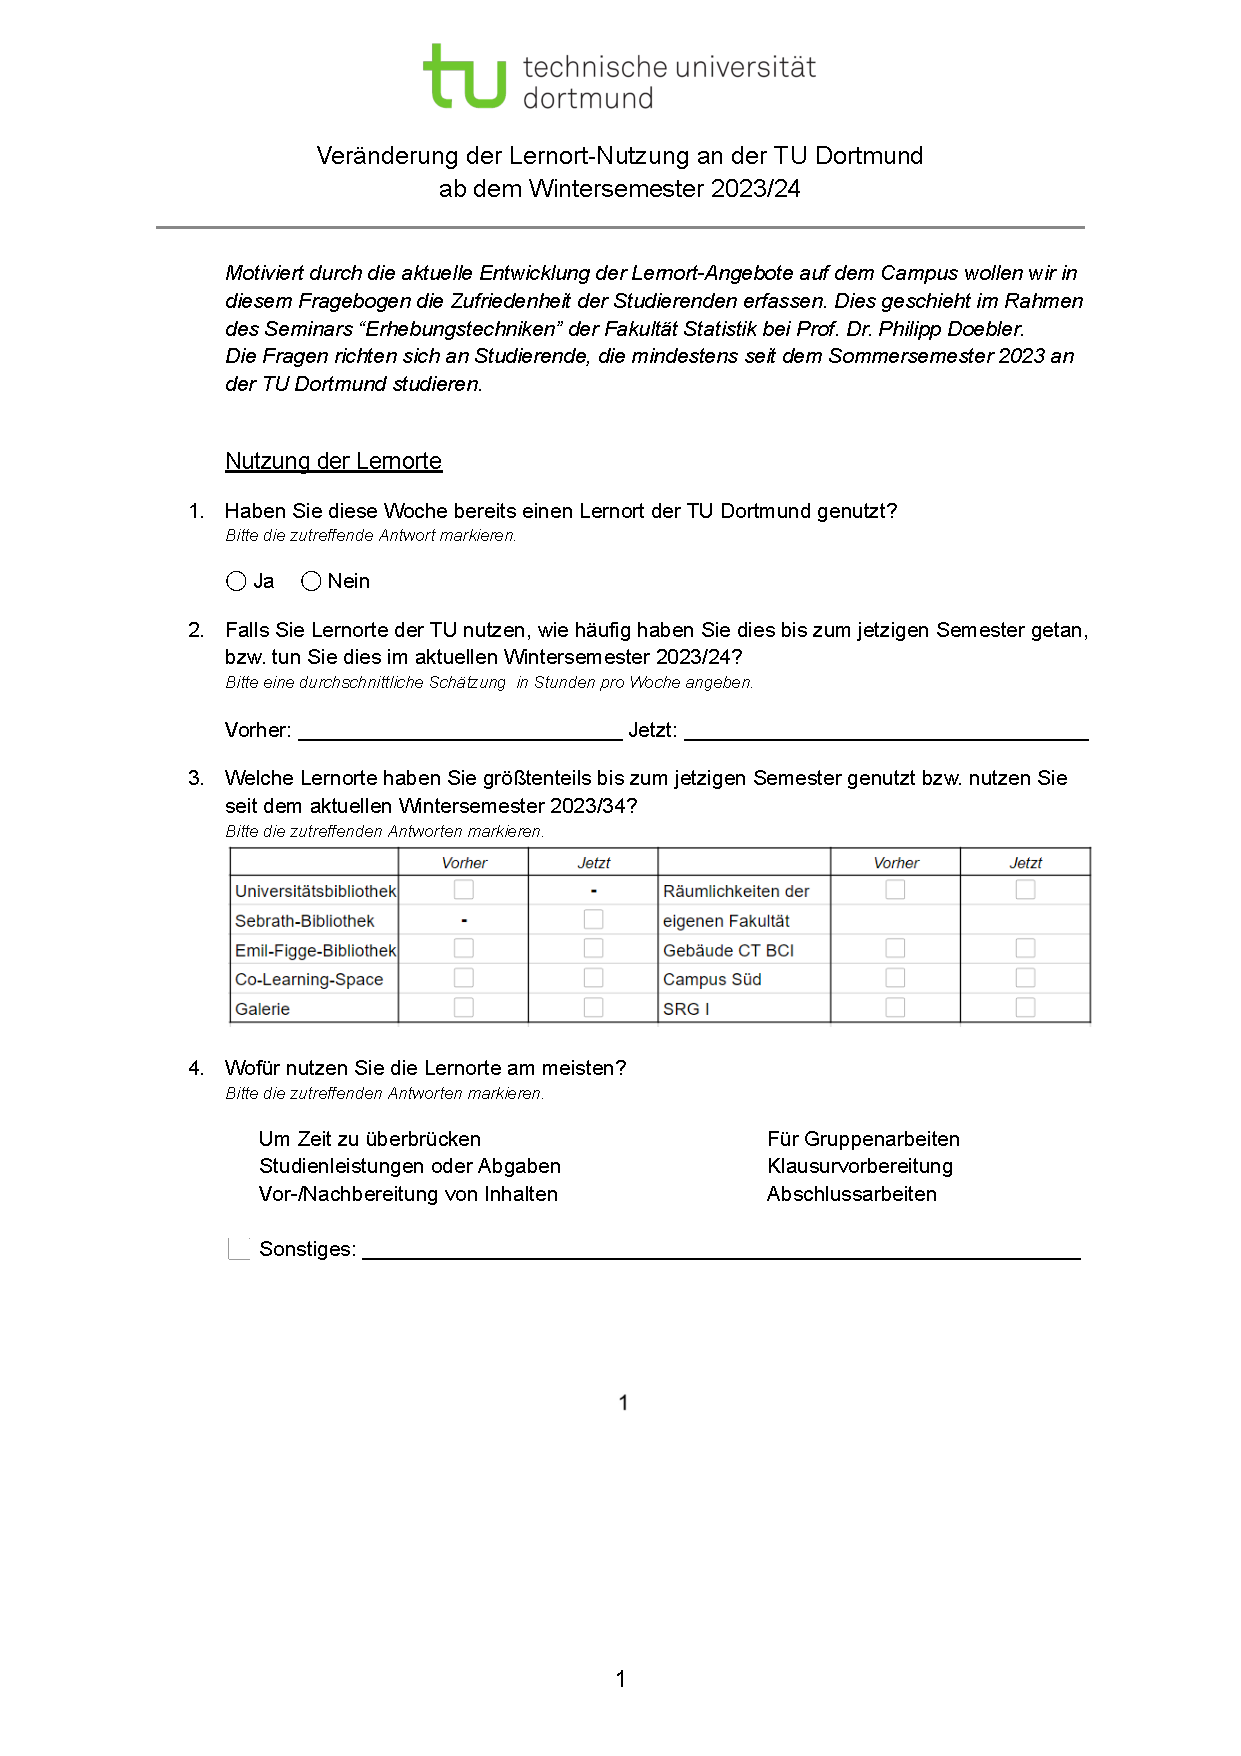
\includepdf[pages=1, offset=0cm -3cm] {Final2.pdf}
\end{figure}
\newpage
\includepdf[pages=2-4] {Final2.pdf}
\newpage
\subsection{Demografie}
\begin{figure}[h]
	\centering
	% Created by tikzDevice version 0.12.5 on 2024-01-27 23:38:32
% !TEX encoding = UTF-8 Unicode
\begin{tikzpicture}[x=1pt,y=1pt]
\definecolor{fillColor}{RGB}{255,255,255}
\path[use as bounding box,fill=fillColor,fill opacity=0.00] (0,0) rectangle (505.89,252.94);
\begin{scope}
\path[clip] (  0.00,  0.00) rectangle (505.89,252.94);
\definecolor{drawColor}{RGB}{0,0,0}
\definecolor{fillColor}{RGB}{0,0,139}

\path[draw=drawColor,line width= 0.4pt,line join=round,line cap=round,fill=fillColor] ( 65.18, 62.61) rectangle (102.87, 76.18);

\path[draw=drawColor,line width= 0.4pt,line join=round,line cap=round,fill=fillColor] (110.41, 62.61) rectangle (148.10,103.32);

\path[draw=drawColor,line width= 0.4pt,line join=round,line cap=round,fill=fillColor] (155.64, 62.61) rectangle (193.33,106.04);

\path[draw=drawColor,line width= 0.4pt,line join=round,line cap=round,fill=fillColor] (200.87, 62.61) rectangle (238.56, 73.47);

\path[draw=drawColor,line width= 0.4pt,line join=round,line cap=round,fill=fillColor] (246.10, 62.61) rectangle (283.79, 70.75);

\path[draw=drawColor,line width= 0.4pt,line join=round,line cap=round,fill=fillColor] (291.33, 62.61) rectangle (329.02,203.75);

\path[draw=drawColor,line width= 0.4pt,line join=round,line cap=round,fill=fillColor] (336.56, 62.61) rectangle (374.25, 81.61);

\path[draw=drawColor,line width= 0.4pt,line join=round,line cap=round,fill=fillColor] (381.79, 62.61) rectangle (419.48, 68.04);

\path[draw=drawColor,line width= 0.4pt,line join=round,line cap=round,fill=fillColor] (427.02, 62.61) rectangle (464.71, 76.18);
\end{scope}
\begin{scope}
\path[clip] (  0.00,  0.00) rectangle (505.89,252.94);
\definecolor{drawColor}{RGB}{0,0,0}

\node[text=drawColor,rotate= 90.00,anchor=base east,inner sep=0pt, outer sep=0pt, scale=  0.67] at ( 86.33, 49.20) {Campus-Süd};

\node[text=drawColor,rotate= 90.00,anchor=base east,inner sep=0pt, outer sep=0pt, scale=  0.67] at (131.56, 49.20) {Galerie};

\node[text=drawColor,rotate= 90.00,anchor=base east,inner sep=0pt, outer sep=0pt, scale=  0.67] at (176.79, 49.20) {SRG-1};

\node[text=drawColor,rotate= 90.00,anchor=base east,inner sep=0pt, outer sep=0pt, scale=  0.67] at (222.02, 49.20) {CLS};

\node[text=drawColor,rotate= 90.00,anchor=base east,inner sep=0pt, outer sep=0pt, scale=  0.67] at (267.25, 49.20) {EF50};

\node[text=drawColor,rotate= 90.00,anchor=base east,inner sep=0pt, outer sep=0pt, scale=  0.67] at (312.48, 49.20) {Mathetower};

\node[text=drawColor,rotate= 90.00,anchor=base east,inner sep=0pt, outer sep=0pt, scale=  0.67] at (357.71, 49.20) {Sebrath};

\node[text=drawColor,rotate= 90.00,anchor=base east,inner sep=0pt, outer sep=0pt, scale=  0.67] at (402.94, 49.20) {Chemiegebäude};

\node[text=drawColor,rotate= 90.00,anchor=base east,inner sep=0pt, outer sep=0pt, scale=  0.67] at (448.17, 49.20) {Mensagebäude};
\end{scope}
\begin{scope}
\path[clip] (  0.00,  0.00) rectangle (505.89,252.94);
\definecolor{drawColor}{RGB}{0,0,0}

\node[text=drawColor,anchor=base,inner sep=0pt, outer sep=0pt, scale=  1.20] at (264.94,224.20) {\bfseries Erhebungsorte};

\node[text=drawColor,rotate= 90.00,anchor=base,inner sep=0pt, outer sep=0pt, scale=  1.00] at ( 10.80,132.47) {Absolute Häufigkeit};
\end{scope}
\begin{scope}
\path[clip] (  0.00,  0.00) rectangle (505.89,252.94);
\definecolor{drawColor}{RGB}{0,0,0}

\path[draw=drawColor,line width= 0.4pt,line join=round,line cap=round] ( 49.20, 62.61) -- ( 49.20,198.32);

\path[draw=drawColor,line width= 0.4pt,line join=round,line cap=round] ( 49.20, 62.61) -- ( 43.20, 62.61);

\path[draw=drawColor,line width= 0.4pt,line join=round,line cap=round] ( 49.20, 89.75) -- ( 43.20, 89.75);

\path[draw=drawColor,line width= 0.4pt,line join=round,line cap=round] ( 49.20,116.89) -- ( 43.20,116.89);

\path[draw=drawColor,line width= 0.4pt,line join=round,line cap=round] ( 49.20,144.03) -- ( 43.20,144.03);

\path[draw=drawColor,line width= 0.4pt,line join=round,line cap=round] ( 49.20,171.18) -- ( 43.20,171.18);

\path[draw=drawColor,line width= 0.4pt,line join=round,line cap=round] ( 49.20,198.32) -- ( 43.20,198.32);

\node[text=drawColor,anchor=base east,inner sep=0pt, outer sep=0pt, scale=  1.00] at ( 37.20, 59.17) {0};

\node[text=drawColor,anchor=base east,inner sep=0pt, outer sep=0pt, scale=  1.00] at ( 37.20, 86.31) {10};

\node[text=drawColor,anchor=base east,inner sep=0pt, outer sep=0pt, scale=  1.00] at ( 37.20,113.45) {20};

\node[text=drawColor,anchor=base east,inner sep=0pt, outer sep=0pt, scale=  1.00] at ( 37.20,140.59) {30};

\node[text=drawColor,anchor=base east,inner sep=0pt, outer sep=0pt, scale=  1.00] at ( 37.20,167.73) {40};

\node[text=drawColor,anchor=base east,inner sep=0pt, outer sep=0pt, scale=  1.00] at ( 37.20,194.87) {50};
\end{scope}
\end{tikzpicture}

	\caption{Verteilung der Erhebungsorte}
\end{figure}

\begin{table}[h]
	\centering
	\begin{tabular}{cl|cc}
		Fakultät & Fachrichtung & Häufigkeit & Anteil \\ \hline
		1 & Mathe & 9 & 6,7\% \\
		2 & Physik & 4 & 2,9\% \\
		3 & Chemie und Chemische Biologie & 1 & 0,7\% \\
		4 & Informatik & 11 & 8,1\% \\
		5 & Statistik & 30 & 22,2\% \\
		6 & Bio- und Chemieingenieurwesen & 5 & 3,7\% \\
		7 & Machinenbau & 5 & 3,7\% \\
		8 & Elektrotechnik und Informationstechnik & 8 & 5,9\% \\
		9 & Raumplanung & 5 & 3,7\% \\
		10 & Architektur und Bauigenieurwesen & 5 & 3,7\% \\
		11 & Wirtschaftswissenschaften & 12 & 8,9\% \\
		12 & \begin{tabular}[l]{@{}l@{}}Erziehungswissenschaften,\\ Psychologie und Bildungsforschung\end{tabular} & 30 & 22,2\% \\
		13 & Rehabilitationswissenschaften & 6 & 4,4\% \\
		14 & Humanwissenschaften und Theologie & 0 & 0\% \\
		15 & Kulturwissenschaften & 2 & 0,15\% \\
		16 & Kunst- und Sportwissenschaften & 2 & 0,15\% \\
		17 & Sozialwissenschaften & 0 & 0\%
	\end{tabular}
	\caption{Verteilung der Fakultäten}
\end{table}
\begin{table}[h]
	\centering
	\begin{tabular}{l|ccc}
		Geschlecht & männlich & weiblich & divers \\ \hline
		Häufigkeit & 66 & 68 & 2
	\end{tabular}
	\vspace{0.5cm}
	\caption{Verteilung der Geschlechtsidentifzierung}
\end{table}
\begin{table}[h]
	\centering
	\begin{tabular}{l|cc}
		angestrebter Abschluss & Bachelor & Master \\ \hline
		Häufigkeit & 117 & 19
	\end{tabular}
	\vspace{0.5cm}
	\caption{Anzahl der Bachelor bzw. Masterstudenten}
\end{table}

\newpage
\subsection{Anteile}
\begin{table}[h]
	\begin{tabular}{l|l}
		Abschnitt                                          & Verantwortliche Person \\ \hline
		Zusammenfassung                                    & Jacqueline Link        \\
		Einleitung                                         & Yannick Miguel         \\
		Erhebungsinstrument                                & Yannick Miguel         \\
		Stichprobe und Datensatz                           &
		Jacqueline Link        \\
		Ergebnisse - Lernortnutzung                        & Jacqueline Link        \\
		Ergebnisse - Wichtigkeit und Umsetzung der Aspekte & Jacqueline Link        \\
		Ergebnisse - Gesamtzufriedeneheit und Score        & Yannick Miguel         \\
		Diskussion                                         & Yannick Miguel         \\
		Reflexion                                          & Jacqueline Link       
	\end{tabular}
\end{table}
\end{document}



